\documentclass{article}
\usepackage[utf8]{inputenc}
\usepackage{geometry}
\usepackage{tabularx}
\usepackage{hyperref}
\usepackage{graphicx}
\usepackage{adjustbox}
\usepackage{multicol}
\usepackage{caption}
\usepackage{subcaption}
\usepackage{xurl}
\usepackage{wrapfig}
\usepackage{float}
\usepackage{enumitem}
\usepackage{makecell}
\usepackage{amsmath}
\usepackage{tikz}
\usepackage{listings}

\geometry{
 a4paper,
 total={170mm,257mm},
 left=20mm,
 top=20mm,
 }

\usetikzlibrary{shapes.geometric, arrows}

\begin{document}
\begin{titlepage}
    \begin{center}
        \vspace*{4cm}

        \hline
        \vspace{.5cm}
        \textbf{\huge Volumetric data structures for real-time ray tracing}
        \vspace{.5cm}
        \hline

        \vspace{1cm}

        
            
            \large Utrecht University\\
            Game and Media Technology\\
            Master thesis\\
            \vspace{.5cm}
            \large In collaboration with Traverse Research.
            

        \vspace{6cm}

        
\includegraphics[width = 8cm]{figures/UU_logo_2021_EN_RGB.png}
        \hfill
        
\includegraphics[width = 5cm]{figures/Traverse+Research+Cropped.png}

        \vspace{1cm}

        \raggedright \textit{Author:} Rosalie de Winther (1326236)\\
        \textit{Company supervisor:} Jacco Bikker\\
        \textit{Primary supervisor:} Alex Telea\\
        \textit{Secondary supervisor:} Peter Vangorp\\
        \today

    \end{center}
\end{titlepage}



\clearpage
\section*{Abstract} \label{abstract}
Volumetric effects such as clouds, explosions, smoke, and fog are important scene elements for computer games. While these can be efficiently handled in a rasterizer, path tracers typically struggle to render them efficiently. This thesis provides the required prior knowledge to think about the different trade-offs of volume data structures, and to provide a specialized implementation for compressed density data. The resulting data structure reduces the voxel data memory footprint by a factor of 8 to 16 times over 16-bit floating point values. This is done by utilizing a novel method of storing density data in block-compressed textures and deduplicating homogeneous nodes. These methods allow us to store animation sequences in game-ready asset sizes and render them at real-time frame rates.
\clearpage
\section*{Acknowledgments} \label{acknowledgments}
\clearpage
\tableofcontents
\clearpage
\section{Introduction} \label{INTRO}
A very basic understanding of rendering in the traditional sense is assumed. Rasterization, the basics of the SIMT execution model and general graphics terms like global illumination are all assumed. In this section we will first provide some foundational knowledge on the topic of ray tracing (Section \ref{INTRO:tracing}). Then we describe the context in which these techniques are implemented at \href{https://traverseresearch.nl/}{Traverse Research} (Section \ref{INTRO:traverse}). Afterwards we explore some of the background research in volume rendering (Section \ref{INTRO:volumes}), how to accelerate it (Section \ref{INTRO:volume_acceleration}) and the current state of the art (Section \ref{INTRO:VDB}). These should provide enough background information to be able to understand this research.

\subsection{Rendering in games} \label{}
\subsubsection{Rasterization} 
\subsubsection{Ray and path tracing} \label{INTRO:tracing}
Rasterization is the rendering technique which has been the industry standard for at least the past 20 years. It involves processing every triangle in the scene. Then, using a set of transforms, these triangles are draw on the screen. Graphics hardware has been built around this pipeline, but it does have limitations. For example, reflections can not show off-screen objects without sophisticated (and often slow) tricks. Ray tracing is an entirely different technique which shoots a ray for every pixel, finds the triangle which intersects that ray, and then shades it. This has the benefit of no longer needing to process every triangle individually, and instead can search for an intersecting triangle quickly. A high level overview of said algorithms can be seen below:

\begin{tabular}{|l|l|}
    \hline
    Technique & Overview\\
    \hline
    Rasterization & \makecell[l]{For each triangle:\\ \quad For each pixel it covers:\\ \qquad Shade} \\
    \hline
    Ray tracing & \makecell[l]{For each pixel:\\\quad Find triangle it intersects:\\ \qquad Shade} \\
    \hline
\end{tabular}

\begin{figure}[H]
    \centering
    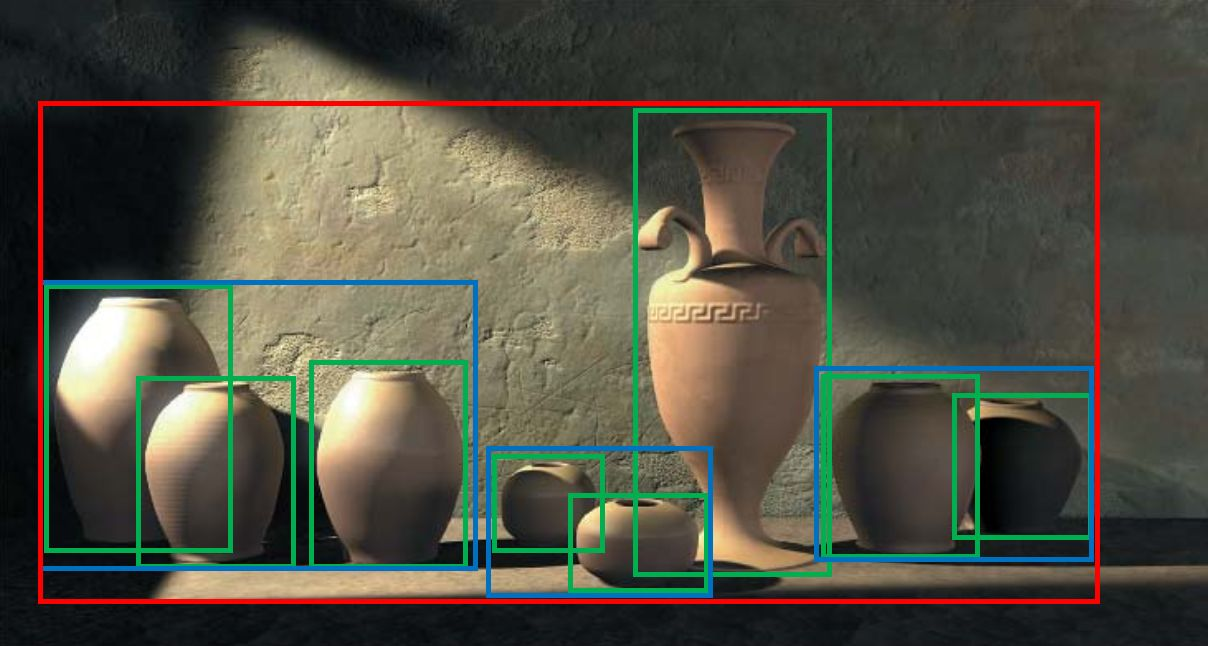
\includegraphics[width=0.9\linewidth]{figures/bvh.jpg}
    \caption{A bounding volume hierarchy where the red bounding box encapsulates all objects. Then a step lower in the hierarchy we see the blue bounding boxes which encapsulate groups of objects. And the leaves, indicated by the green bounding boxes, contain the primitives. These structures are stored in a tree like structure and can, theoretically, have infinite depth or width. Finding the intersection between a ray and the bounding volume hierarchy can be done in $O(\log n)$ time on average, where n is the number of primitives. \cite{BVHJacco}}
    \label{fig:bvh}
\end{figure}

Although ray tracing has been theorized by many to be the replacement of classic rasterization methods, we have only recently seen it being applied to games after NVIDIA released its RTX graphics cards. Additionally, we see that all AAA games currently still depend on the rasterizer and only use ray tracing to enhance their graphics either by adding realistic (1) diffuse indirect light, which is often mislabeled as GI, (2) shadows, (3) reflections, (4) ambient occlusion or a combination of these four\cite{NVIDIARTX}. 

Path tracing is a specific algorithm which uses ray tracing to calculate physically accurate images by trying to solve the rendering equation \cite{kajiya1986rendering}. It does this by recursively performing a Monte Carlo experiment over the integral in the rendering equation for every pixel. This results in a realistic image once converged. However, for the longest time this has been too slow to run in real-time on commodity hardware. Fortunately, there have been some major advances in (1) sampling techniques as described in \cite{lin2022generalized} and (2) filtering techniques as described in \cite{yang2020survey}. Along with the advent of better GPU hardware, it might make real-time path tracing a reality for upcoming AAA games. 

Generally, path tracing involves multiple steps to achieve real time performance \cite{laine2013megakernels}, (1) ray generation, (2) ray extension, (3) shading and (4) shadow ray extension. This pipeline is executed for every pixel on screen, so for a standard 1080p monitor that would be $1920*1080=2.073.600$ rays. Step 1 is executed once at the start, and then the latter three steps are done repeatedly to simulate realistic light transport through the scene. The main task of steps 2 and 4 is to find an intersections with the scene geometry. This can be done by individually performing intersection tests with every triangle in the scene with a time complexity of $O(n)$, where $n$ is the number of triangles. However, this linear scaling is prohibitive when the complexity of models increases. So to fix this problem, bounding volume hierarchies (BVH as seen in Figure \ref{fig:bvh}) are used to accelerate these intersection tests. This is done by creating a traversable tree with triangles at the leaf nodes, which reduces the average traversal time to  $O(\log n)$. To allow instanced rendering without drastically increasing the triangle count of the scene or increasing build times, a top level acceleration structure (TLAS) is created over a bottom level acceleration structure (BLAS). Here the TLAS contains pointers to multiple BLAS's which contain the actual model data \cite{VulkanAccelerationStructures}. 

\subsection{Volume rendering} \label{INTRO:volumes}
In this project volume data represents clouds, explosions, fire and sand/dust storms. This means that we are not just interested in finding the boundary of a volume, but also in the contents of the volume. We may have varying densities or even different materials within one volume. For example, a flame which emits light surrounded by smoke, where the outer edge of this smoke is so sparse that it is almost completely transparent. When shading these kinds of materials there are three main things which can happen: (1) The ray is absorbed, meaning that no light transport will be rendered. When this happens, the light energy is converted into another energy form like heat. (2) The ray is traversed through or bounces off the particle. This will change the direction of the ray and potentially change the ray payload, for example when a blue particle is hit, the ray is modified to only return the blue color if a light is hit. (3) The ray hits an emissive particle. Meaning that light transport will be rendered, and the ray will not continue.

Ray tracing these kinds of volumes is very different from normal ray tracing, as they require completely different methods. Normally there is a set of surfaces which define a scene. To render these scenes, BVH's are used to find an intersection between a ray and the scene as described in Section \ref{INTRO:tracing}. For volume rendering we don't have these concrete surfaces but instead have volumes with implicit particles, like dust or water droplets from a cloud. To render these volumes we somehow have to find where we hit such a particle and evaluate its shading function. We do not simulate these particles individually but describe volumes of the scene using densities, which are discretized into small volumetric pixels (voxels). When traversing such a volume we calculate how far we can traverse through these densities before we are likely to hit a particle. Then we take the step, evaluate the shading function and calculate how long our next step can be. This process is called ray marching \cite{RenderingWithTwoTriangles}. For homogeneous volumes (with a uniform density) these step sizes will always be the same, but for heterogeneous volumes they might not. In the heterogeneous case we calculate the longest possible step we could take through the most dense voxel in our scene and use that to make sure we do not overshoot and miss any dense voxels. This method quickly becomes prohibitively expansive when a single voxel has a high density. A solution would be to take steps proportional to the highest local density, for example the highest density of the $8^3$ nearest voxels. This way we can take step sizes which are proportional to the densities which we are more likely to traverse, instead of crippling the performance for every ray because of a single voxel \cite{kutz2017spectral}.

\begin{figure}[H]
    \centering
    
\includegraphics[width=0.9\linewidth]{figures/sample_step_size.png}
    \caption{A ray traversing through a heterogeneous volume, where dots represent the location of shading evaluations. As can be seen, the more dense the volume (darker) the shorter the steps are.}
    \label{fig:sample_step_size}
\end{figure}

\subsection{Traverse Research} \label{INTRO:traverse}
\href{https://traverseresearch.nl/}{Traverse Research} is a company which does state-of-the-art research in graphics, and more specifically ray tracing. Their current in-house hybrid rendering framework "Breda" includes many features which are expected from a modern renderer. However, volume rendering is still largely unexplored. Breda can compile for either a Vulkan or a DirectX 12 backend to make use of the latest ray tracing features. Along with that, some advanced rendering techniques are used. Most notably bindless rendering\cite{BindlessRenderingSetup} and render graphs\cite{RenderGraph101}. The former is a different way of interfacing with data on the GPU, while the latter simplifies GPU synchronization while optimizing dispatch ordering based on read and write dependencies of different pieces of data on the GPU. All of this is written in Rust and HLSL, which this project must adhere to. 

At \href{https://traverseresearch.nl/}{Traverse} there is another parallel project which involves volumetrics. That project focuses on shading as explained in Section \ref{INTRO:volumes}. Merging the shading with the result of this project should allow for physically based shading with fast volume traversal in order to perform real-time realistic volumetric rendering. The exact placement of this project inside the Breda framework can be seen in Figure \ref{fig:project_structure}.

\begin{figure}[H]
    \centering
    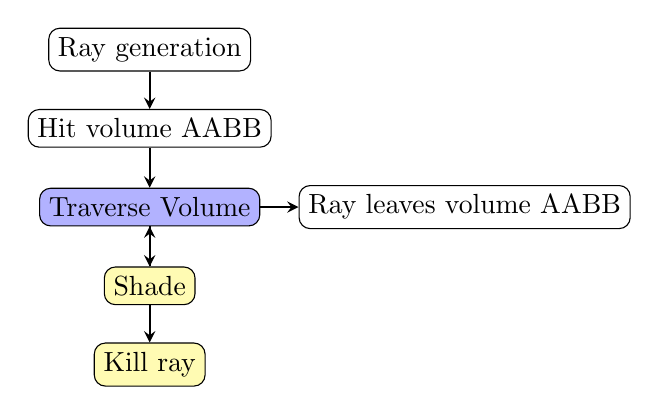
\begin{tikzpicture}[node distance=1cm]
    \tikzstyle{arrow} = [thick,->,>=stealth]
    \tikzstyle{done} = [rectangle, rounded corners, minimum width=1cm, minimum height=0.33cm,text centered, draw=black]
    \tikzstyle{this} = [rectangle, rounded corners, minimum width=1cm, minimum height=0.33cm,text centered, draw=black, fill=blue!30]
    \tikzstyle{other} = [rectangle, rounded corners, minimum width=1cm, minimum height=0.33cm,text centered, draw=black, fill=yellow!30]
    \node (start) [done] {Ray generation};
    \node (aabb) [done, below of=start] {Hit volume AABB};
    \node (trav) [this, below of=aabb] {Traverse Volume};
    \node (shade) [other, below of=trav] {Shade};
    \node (kill) [other, below of=shade] {Kill ray};
    \node (leaves) [done, right of=trav, xshift=3cm] {Ray leaves volume AABB};

    \draw [arrow] (start) -- (aabb);
    \draw [arrow] (aabb) -- (trav);
    \draw [arrow] (trav) -- (shade);
    \draw [arrow] (trav) -- (leaves);
    \draw [arrow] (shade) -- (trav);
    \draw [arrow] (shade) -- (kill);
    
    \end{tikzpicture}
    \caption{Flow diagram of the volume rendering project inside \href{https://traverseresearch.nl/}{Traverse}. The white boxes indicate parts of the pipeline which already exist inside the Breda framework. The blue box shows what this project will focus on, and the yellow boxes highlight what parts are happening in parallel with this project. As can be seen, when rays bounce inside a volume, they can repeatedly be shaded and continue traversal until they either leave the volume or are killed because they wont contribute any light to the scene.}
    \label{fig:project_structure}
\end{figure}

\subsection{Accelerating volume traversal} \label{INTRO:volume_acceleration}
Data structures for heterogeneous volumes have seen multiple forms trying to optimize ray marching performance, memory footprint, update speed and simplicity. As described in Section \ref{INTRO:volumes}, this project specifically targets heterogeneous volumes which often consist of gradients where outer voxels can have small non-zero values, instead of having opaque volume boundaries. This might alter the effectiveness of certain methods or require reducing the precision of our data in favor of traversal speed. For example, we could compress a set of voxels which have similar density values into a single larger voxel with the averaged density. This will make the data structure lossy but might significantly improve traversal speed or memory footprint. We will briefly go over some of the major volume data structures, below. 

\noindent\textbf{Flat 3D array:} The most basic structure (see Figure \ref{fig:dda_traversal}). Here, every value in the 3D array corresponds to a voxel. Indexing into this structure is fast and editing is trivial. However, there is no compression or empty space skipping. All rays might have to step through the entire volume one step at a time (which is often done using the Digital Differential Analyzer (DDA) algorithm \cite{amanatides1987fast}) which does not scale well to volumes with larger resolutions. Another problem with flat arrays is their memory requirement as it has cubic scaling with the resolution. However, small scale simulation software still often relies on this data structure as it is easy to implement, and in many cases simulations have to update each voxel anyway.

\begin{figure}[H]
    \centering
    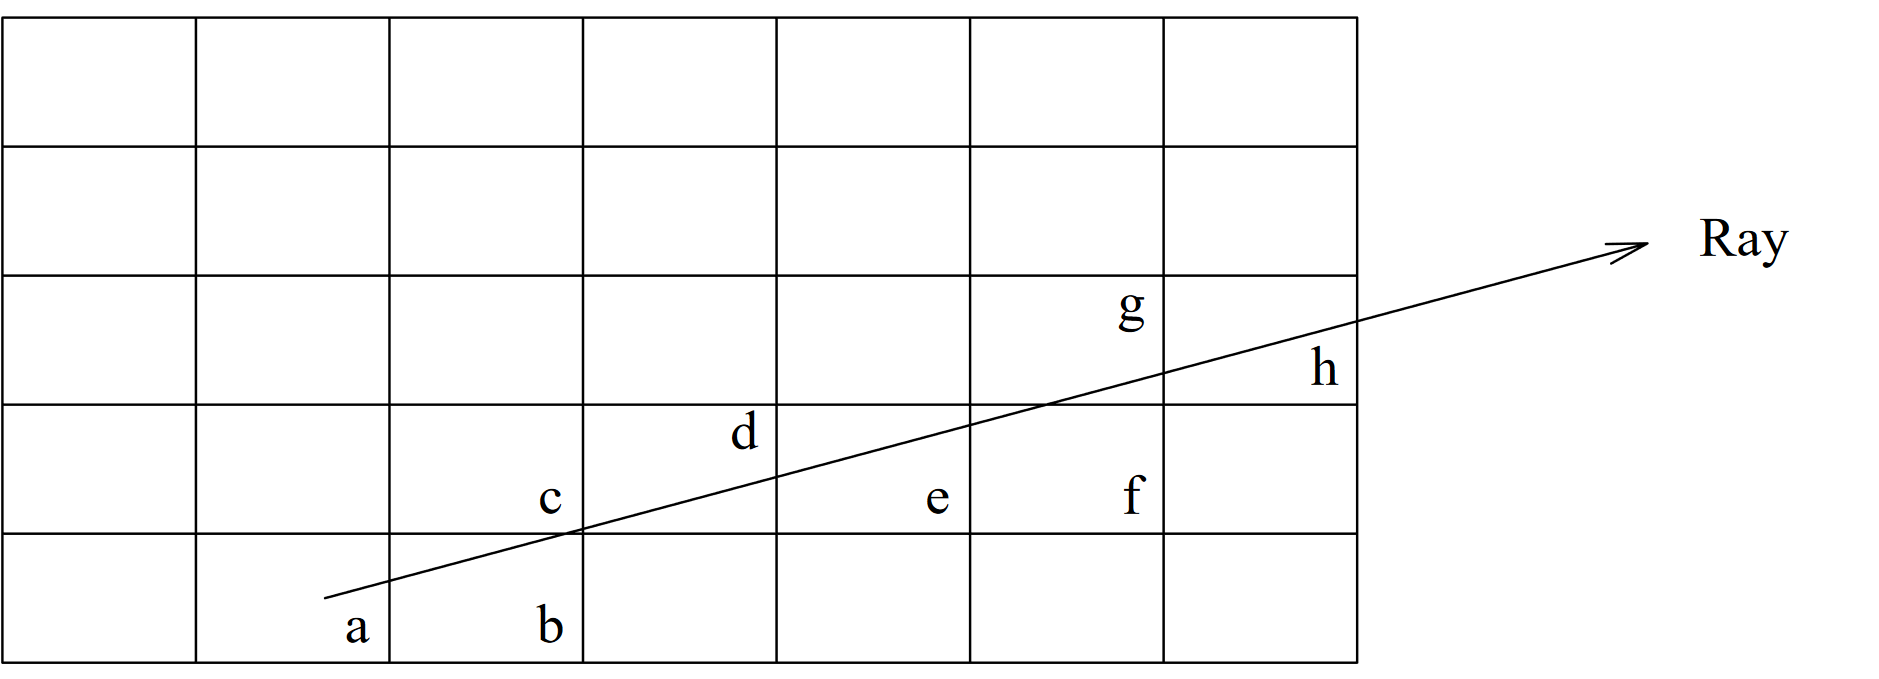
\includegraphics[width=0.9\linewidth]{figures/dda.png}
    \caption{DDA traversal through a flat grid. Step through every voxel that intersects the ray. \cite{amanatides1987fast}}
    \label{fig:dda_traversal}
\end{figure}

\noindent\textbf{Efficient Sparse Voxel Octrees (ESVO):} A solution to the memory problems was proposed by NVIDIA, by introducing sparsity to homogeneous volume data \cite{laine2010efficient}. The main contribution is a data structure which drastically reduces the memory footprint by not storing information about homogeneous areas. This memory reduction also yields a speedup when traversing the volume, as larger steps can be taken through homogeneous areas (see Figure \ref{fig:esvo}). Along with that, the structure will more easily fit in the different caches of the GPU. However, due to the nature of tree structures, the data access pattern is less coherent which negatively impacts ray marching performance. The paper also did not take any form of animation into account. So this data structure only really works on static scenes \cite{JohnLinPerfectEngine}. 

\begin{figure}[H]
    \centering
    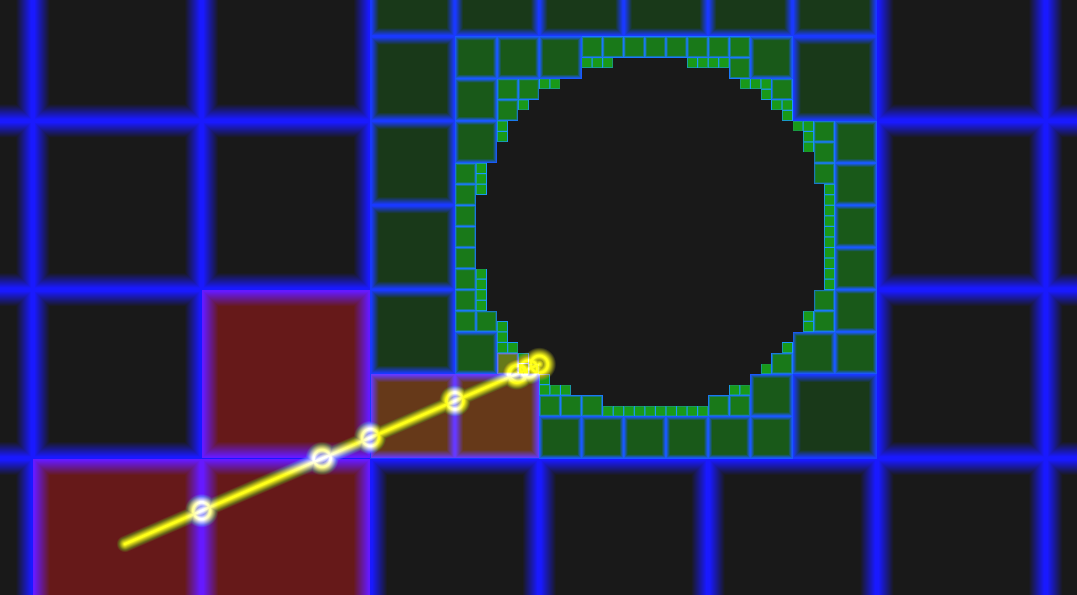
\includegraphics[width=0.9\linewidth]{figures/esvo_traversal.png}
    \caption{Hierarchical DDA traversal through a sparse voxel octree. The yellow line is our ray. The brighter green a cell is, the deeper our nodes in the octree are. We can see that nodes which are further away from the circle, can be stepped through with big steps, but as we approach the circle, our steps become smaller. Image obtained from Shadertoy.}
    \label{fig:esvo}
\end{figure}

\noindent\textbf{High Resolution Sparse Voxel DAGs (SVDAG):} A follow-up paper was released further improving the memory footprint optimization \cite{kampe2013high}. Here, the nodes of the octree can be reused for identical volumes, so one leaf can be the child of multiple nodes that share the same data (see Figure \ref{fig:DAG_node_deduplication}). The result is a significant reduction in memory usage over ESVO. Afterward, additional papers were written to, (1) further optimize the memory footprint by creating a lossy data structure which will slightly alter the volume data in an attempt to find more similar volumes \cite{van2020lossy} (LSVDAG). And (2) allow for real time editing of this data structure \cite{careil2020interactively} (HashDAG). 

\begin{figure}[H]
    \centering
    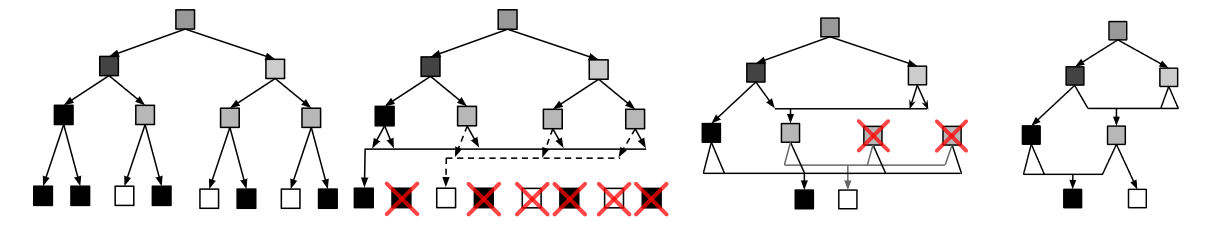
\includegraphics[width=0.9\linewidth]{figures/DAG_node_deduplication.png}
    \caption{Removal of identical nodes in all levels of a binary tree. In the SVDAG paper the same technique is applied to octrees. \cite{kampe2013high}}
    \label{fig:DAG_node_deduplication}
\end{figure}

\noindent\textbf{Brickmaps:} Later another paper was released which tried to maintain part of the memory benefits from octrees while also improving ray marching performance \cite{van2015real}. This was done by keeping the idea of a hierarchical structure, but limiting the tree depth to 2 layers (a top level grid, the brickmap and the bottom level bricks, as can be seen in Figure \ref{fig:brickmap}), which improves cache utilization. An additional benefit of reducing the depth of a data structure is the update time. When running a fluid simulation, which has to touch every leaf node in a tree, a shallower tree will take fewer steps when going down to bottom of the tree to modify each voxel. Similar to the flat 3D array, the brickmap structure is quite fast when it comes to update speeds, as both have very shallow tree structures. Another paper explores implicit brickmaps \cite{niessner2013real}. These are implicit because they dont encode their location in a grid, but hash a world position and use that hash to index into the brick buffer directly. This allows for an unbounded index space instead of having to create a grid inside a certain axis aligned bounding box (AABB). However, nothing has been documented about them in the context of ray tracing.

\begin{figure}[H]
    \centering
    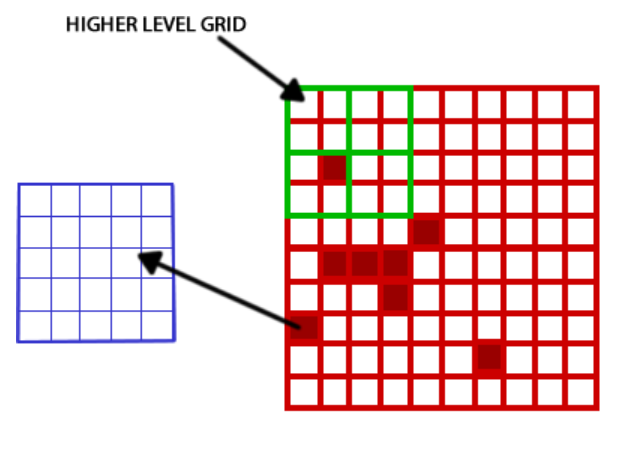
\includegraphics[width=0.9\linewidth]{figures/brickmap.png}
    \caption{Here we see the brickmap (in red), which is dense. And whenever an area in this brickmap is not homogeneous (indicated by the filled in squares), we point to a brick (in blue). \cite{van2015real}}
    \label{fig:brickmap}
\end{figure}

\noindent\textbf{Signed distance fields (SDF):} Recently, NVIDIA has done research about using SDFs to speed up traversal\cite{soderlund2022ray}. The general idea behind these distance fields is that the maximum step length a ray could take in any direction (without hitting anything) is pre-calculated, and used to skip over voxels that are known to be empty (see Figure \ref{fig:SDF_marching}). This method could be applied to most of the techniques described above, and might specifically be promising when combined with flat structures which dont implicitly store distance values by using bigger nodes in homogeneous volumes. However, calculating these SDF's is one additional step in the pipeline. Although this can be done quickly even for large volumes (less than $1$ ms for $1024^3$ voxels \cite{cao2010parallel}), it is unclear if the speedup during tracing outweighs the construction cost. Some other results from NVIDIA's paper are related to the new ray tracing graphics cards. These cards have hardware dedicated specifically to AABB and triangle intersections, and thus traversal algorithms which use these calculations can be sped up. In the paper, they did test storing bricks into a BVH, then traversing the BVH and using DDA to traverse through the bricks. Another, more interesting result they found was that storing every single voxel in a BVH actually had the fastest traversal speed. This last method makes very efficient use of the fixed function BVH traversal of the ray tracing cards, at the cost of a very large BVH.

\begin{figure}[H]
    \centering
    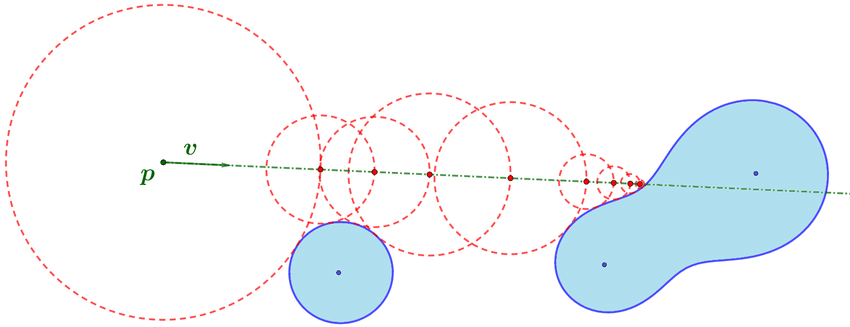
\includegraphics[width=0.9\linewidth]{figures/sdf_ray_marching.png}
    \caption{Marching through a signed distance field enables steps which are exactly as long, as the closest heterogeneity is far away. Here we see the ray in green, and the step sizes are indicated by the red circles. \cite{SDF_sphere_marching}}
    \label{fig:SDF_marching}
\end{figure}

\subsection{VDB}\label{INTRO:VDB}
In the movie industry, \textbf{VDB} \cite{museth2013vdb} has been the standard for volumetric rendering for a long time. This is a hierarchical B+tree structure with 3 layers (see Figure \ref{fig:VDB}), which optimizes for both query speed and memory size. It does so by making clever use of bitmasks, logical bitwise operations and inverted tree traversal. The last of these optimizations means that we don't have to traverse down the tree every time we query a point. But instead we assume that consecutive points will be close to each other, and remember where we are in the tree. Then the next time we query a point we start at the bottom of the tree and have $O(1)$ access time if we retrieve a point which resides in the same bottom layer. 

The VDB structure has mostly been used on the CPU. There have been implementations which port VDB to the GPU, but these do not support dynamic topology \cite{hoetzlein2016gvdb} \cite{museth2021nanovdb}. They would allow individual voxels to be modified, but can't place new voxels in arbitrary locations. This limitation makes simulation on the GPU impractical while maintaining the sparsity which makes the structure effective. The reason why this dynamic topology has never been implemented likely has to do with an inherent race condition when trying to modify any tree structure in parallel.

Research has also been conducted on encoding voxels or even internal layers of the VDB structure in neural networks \cite{kim2022neuralvdb}. These neural encodings can store a lot of detail in very limited memory, but take minutes to train. Which, again, makes dynamic updates impossible.

One very useful result of the standardization of VDB technology is the data format. Many tools can interface directly with the VDB file format \cite{VDBADeepDive}, and many artistic tools can export to the VDB file format. These features make it easy to download specific effects and test in a specific renderer.

\begin{figure}[H]
    \centering
    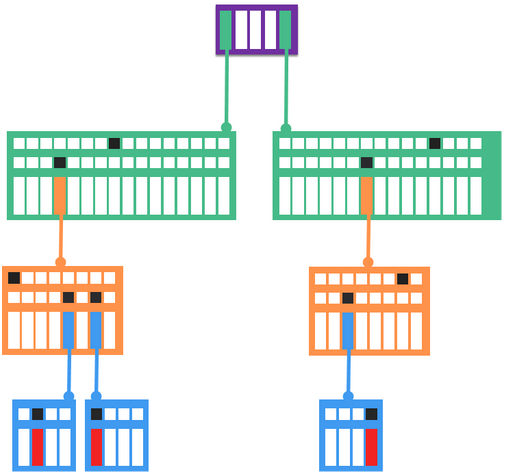
\includegraphics[width=0.9\linewidth]{figures/OpenVDB.png}
    \caption{The four level tree structure of the VDB data structure. In purple we see the top node which has arbitrary size and points to the first level of internal nodes. The two levels of internal nodes (in green and orange) both contain three rows of values. The top row is a bitmask indicating which values are "active" (this is application specific), the middle row is a bitmask indicating that a child node exists, and the bottom row containing a pointer to the child node. Then in blue we have a top row which is a bitmask indicating if a voxel is empty, and the bottom row containing the actual voxel data. \cite{museth2013vdb}}
    \label{fig:VDB}
\end{figure}

\subsection{Gaps in current research}\label{INTRO:GAPS}
To conclude the introduction we will now list the most notable issues with the current state-of-the-art, and how we can push the state-of-the-art forward in a meaningful way. Many methods have either optimized volume data structures for memory usage (ESVO, SVDAG), ray tracing performance (Brickmaps, signed distance fields) or simulation times (flat 3D array). However none of these techniques currently can do all three of these things while keeping all data and computation on the GPU. For our purposes we require an extension to the VDB data structure to enable dynamic topology on the gpu. Furthermore, combining VDB with the compression scheme of SVDAG can be explored to allow for efficient animation playback. Additionally, the combination of signed distance fields can be incorporated into the VDB structure to allow for faster ray marching through these volumes.
\clearpage
\section{Related work} \label{related_work}
This section goes over all prior knowledge that is required to properly follow the rest of this thesis. We quickly go through some fundamentals of rendering, and quickly move to volume rendering specific topics. We conclude this section with the gaps in current research and where this research fits in.



\begin{wrapfigure}{r}{0.4\textwidth}
    \centering
    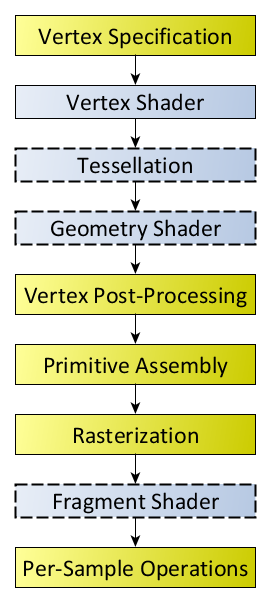
\includegraphics[width=0.5\linewidth]{figures/rasterization_pipeline.png}
    \caption{An overview of the rasterization pipeline, where blue stages are programmable and yellow stages are dedicated stages built into GPU hardware. We start with a bunch of vertices and apply a vertex shader. This allows the triangles to be transformed for whatever reason, whether it's because the camera was moved or an object has changed for example. Then we tessellate the vertices into triangles. After which we apply an optional geometry shader that can generate or remove triangles. Then our triangles are projected onto an image, and we end up with information like normal, texture coordinate, and depth. This information can then be used to calculate the final color of a certain set of pixels. \cite{RasterPipeline}}
    \label{fig:rasterization_pipeline}
\end{wrapfigure}


\subsection{Rendering in games} \label{related_work:rendering}
Computers have existed for some time now, and since the start, they have been used to render things on a screen. Whether this is text, graphs, photos, or virtual worlds. When rendering virtual worlds, for example, games or movies, optimized algorithms have to be used to keep up with the growing complexity and increasing fidelity that is expected of new titles. One of these algorithms that has been used in practically all games is rasterization, which quickly projects triangles onto the screen. A different algorithm, with different benefits and drawbacks, is ray tracing, which tries to emulate the physical properties of light as it exists in the real world. Usually, we render scenes that consist of a set of models, for example for every tree, rock or character in the world. These models are made up of triangles which store details such as material, normal and position.


\subsubsection{Rasterization} \label{related_work:rendering:rasterization}
Screen space rendering techniques using the graphics processing unit's (GPU) hardware rasterizer are frequently referred to as rasterization. This technique has been the industry standard for at least the past 20 years. It is a pipeline of operations that calculates which triangles are visible (see Figure \ref{fig:rasterization_pipeline}). Because graphics hardware has been optimized for this specific pipeline, it is fast and thus, if possible, the rasterization pipeline can and should be exploited where possible. However, there are issues. For example, reflections can not show off-screen objects without sophisticated (and often slow) tricks. This is an inherent issue with the rasterization because the fragment shader stage does not know anything about off-screen and obscured triangles. Along with that, rasterization performance scales linearly with the number of triangles. Therefore, it quickly becomes impractical to use for scenes/assets with incredibly high triangle counts, as required by modern render pipelines.

\subsubsection{Ray and path tracing} \label{related_work:rendering:ray_tracing}
Ray tracing is an entirely different technique that allows us to create arbitrary rays and find what primitives they intersect. Which has the benefit of no longer being bound to a certain view matrix, like with rasterization. This immediately opens up the door for techniques that were traditionally not possible. For example, off-screen reflections can now be rendered by shooting new rays from the reflection point (see Figure \ref{fig:path_ray_raster}). We also don't have to process every triangle individually, instead, we can shoot rays for every pixel in the screen, and find the intersecting triangles quickly.

Although ray tracing has been theorized by many to be the replacement of classic rasterization methods, we have only recently seen it being applied to games after NVIDIA released its RTX graphics cards. Additionally, we see that all AAA games currently still depend on the rasterizer and only use ray tracing to enhance their graphics either by adding realistic (1) diffuse indirect light, which is often mislabeled as global illumination, (2) shadows, (3) reflections, (4) ambient occlusion or a combination of these four\cite{NVIDIARTX}.
\begin{figure}[H]
    \centering
    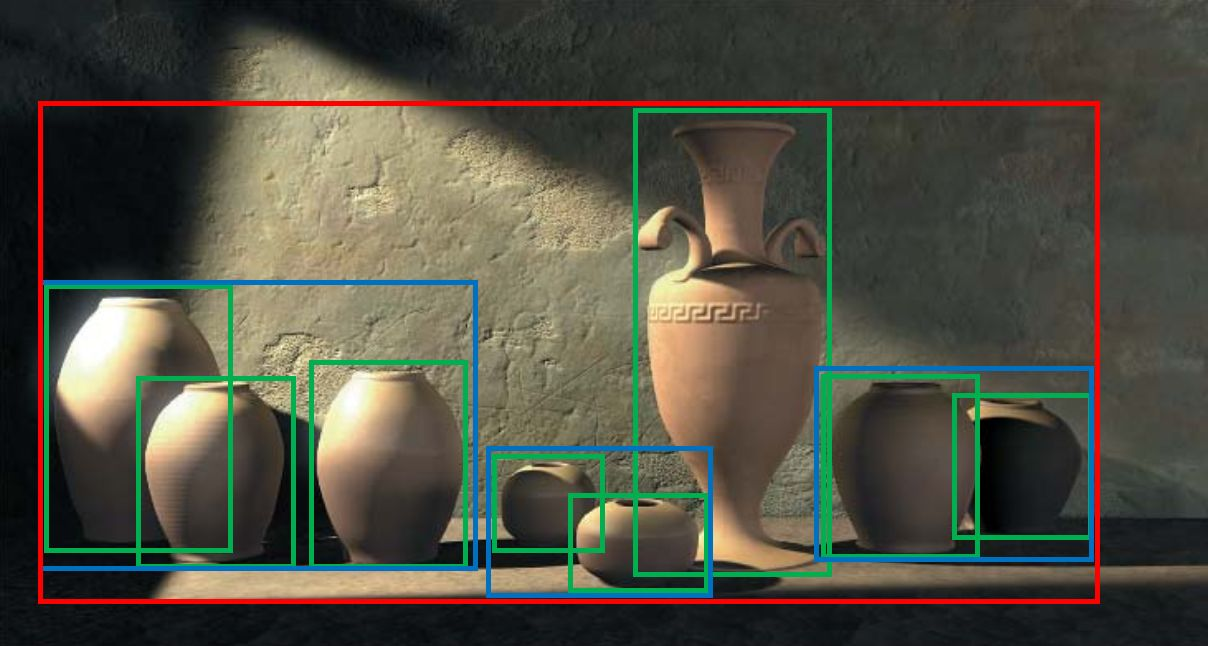
\includegraphics[width=0.9\linewidth]{figures/bvh.jpg}
    \caption{A bounding volume hierarchy where the red bounding box encapsulates all objects. Then a step lower in the hierarchy, we see the blue bounding boxes which encapsulate groups of objects. And the leaves, indicated by the green bounding boxes, contain the primitives. These structures are stored in a tree-like structure and can, theoretically, have infinite depth or width. Finding the intersection between a ray and the bounding volume hierarchy can be done in $O(\log n)$ time on average, where n is the number of primitives. \cite{BVHJacco}}
    \label{fig:bvh}
\end{figure}

Path tracing is a specific algorithm that uses ray tracing to calculate physically accurate images by trying to solve the rendering equation \cite{kajiya1986rendering}. It does this by using recursive numerical integration of the rendering equation for every pixel. This results in a realistic image once converged. However, for the longest time, this has been too slow to run in real-time on commodity hardware. Fortunately, there have been some major advances in (1) sampling techniques as described in \cite{lin2022generalized} and (2) filtering techniques as described in \cite{yang2020survey}. Along with the advent of better GPU hardware, it might make real-time path tracing a reality for upcoming AAA games.

\begin{wrapfigure}{r}{0.4\textwidth}
    \centering
    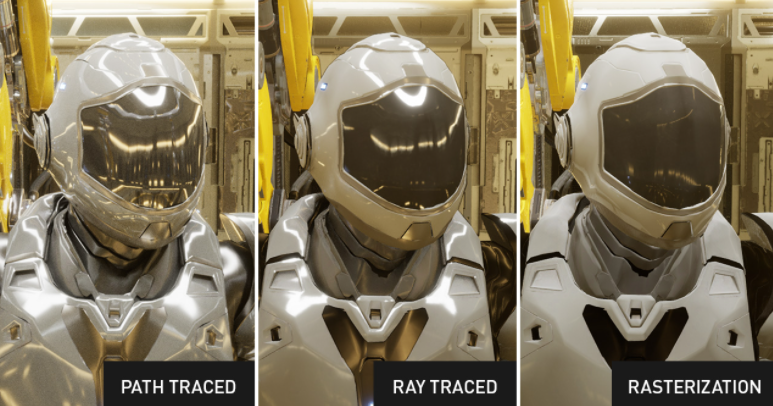
\includegraphics[width=\linewidth]{figures/nvidia_ray_path_rasterization.png}
    \caption{Here we see the difference between a path traced, a ray-traced and a rasterized render. As can be seen, the rasterized scene does not contain accurate reflections and has trouble with specular highlights from the many lights. The ray-traced render does show accurate specular reflections. And when we look at the path traced scene we also see glossy reflections and accurate indirect illumination. \cite{NVIDIAPathRayRaster}}
    \label{fig:path_ray_raster}
\end{wrapfigure}

Generally, path tracing involves multiple steps to achieve real-time performance \cite{laine2013megakernels}, (1) ray generation, (2) ray extension, (3) shading and (4) shadow ray extension. This pipeline is executed for every pixel on the screen, so for a standard 1080p monitor that would be $1920*1080=2.073.600$ rays. Step 1 is executed once at the start, and then the latter three steps are done repeatedly to simulate realistic light transport through the scene. The main task of steps 2 and 4 is to find intersections with the scene geometry. This can be done by individually performing intersection tests with every triangle in the scene with a time complexity of $O(n)$, where $n$ is the number of triangles. However, this linear scaling is prohibitive when the complexity of models increases. So to fix this problem, bounding volume hierarchies (BVH as seen in Figure \ref{fig:bvh}) are used to accelerate these intersection tests. This is done by creating a traversable tree with triangles at the leaf nodes, which reduces the average traversal time to  $O(\log n)$. To allow instanced rendering without drastically increasing the triangle count of the scene or increasing build times, a top-level acceleration structure (TLAS) is created over a bottom-level acceleration structure (BLAS). Here the TLAS contains pointers to multiple BLAS's which contain the actual model data \cite{VulkanAccelerationStructures}.

\subsection{Path traced volume rendering} \label{related_work:path_traced_volume_rendering}
In this project volume data represents clouds, explosions, fire and sand/dust storms. This means that we are not just interested in finding the discretized boundary of a volume, but also in the contents of the volume. We may have varying densities or even different materials within one volume. For example, a flame that emits light surrounded by smoke, where the outer edge of this smoke is so sparse that it is almost completely transparent. When shading these kinds of materials there are three main things which can happen: (1) The ray is absorbed, meaning that no light transport will be rendered. When this happens, the light energy is converted into another energy form like heat. (2) The ray is traversed through (refracted) or bounces off (reflected) the particle. This will change the direction of the ray and potentially change the ray payload, for example when a blue particle is hit, the ray is modified to only return the blue color if a light is hit. (3) The ray hits an emissive particle. Meaning that light transport will be rendered, and the ray will not continue.

\subsubsection{Data structure} \label{related_work:path_traced_volume_rendering:data_structure}
Ray tracing these kinds of volumes is different from normal ray tracing, as they require completely different methods. Normally there is a set of surfaces that define a scene. To render these scenes, BVHs are used to find an intersection between a ray and the scene as described in Section \ref{related_work:rendering:ray_tracing}. For volume rendering, we don't have these concrete surfaces but instead have volumes with implicit particles, like dust or water droplets from a cloud. To render these volumes we somehow have to find where we hit such a particle and evaluate its shading function. We do not simulate these particles individually but describe volumes of the scene using densities, which are discretized into small volumetric pixels (voxels).

\subsubsection{Delta tracking} \label{related_work:path_traced_volume_rendering:delta_tracking}
When traversing such a volume we calculate how far we can traverse through these densities before we are likely to hit a particle. Then we take the step, evaluate the shading function and calculate how long our next step can be. This process is called ray marching \cite{RenderingWithTwoTriangles}. For homogeneous volumes (with a uniform density) these step sizes will always be the same, but for heterogeneous volumes, they might not. In the heterogeneous case, we calculate the longest possible step we could take through the most dense voxel in our scene and use that to make sure we do not overshoot and miss any dense voxels. This method is called delta tracking \cite{kutz2017spectral} and quickly becomes expansive when a single voxel has a high density. A solution would be to take steps proportional to the highest local density, for example, the highest density of the $8^3$ nearest voxels. This way we can take step sizes that are proportional to the densities which we are currently traversing, instead of crippling the performance for every ray because of a single voxel.

\begin{figure}[H]
    \centering
    
\includegraphics[width=0.9\linewidth]{figures/sample_step_size.png}
    \caption{A ray traversing through a heterogeneous volume, where dots represent the location of shading evaluations. As can be seen, the more dense the volume (darker) the shorter the steps are.}
    \label{fig:sample_step_size}
\end{figure}

\begin{wrapfigure}{r}{0.4\textwidth}
    \centering
    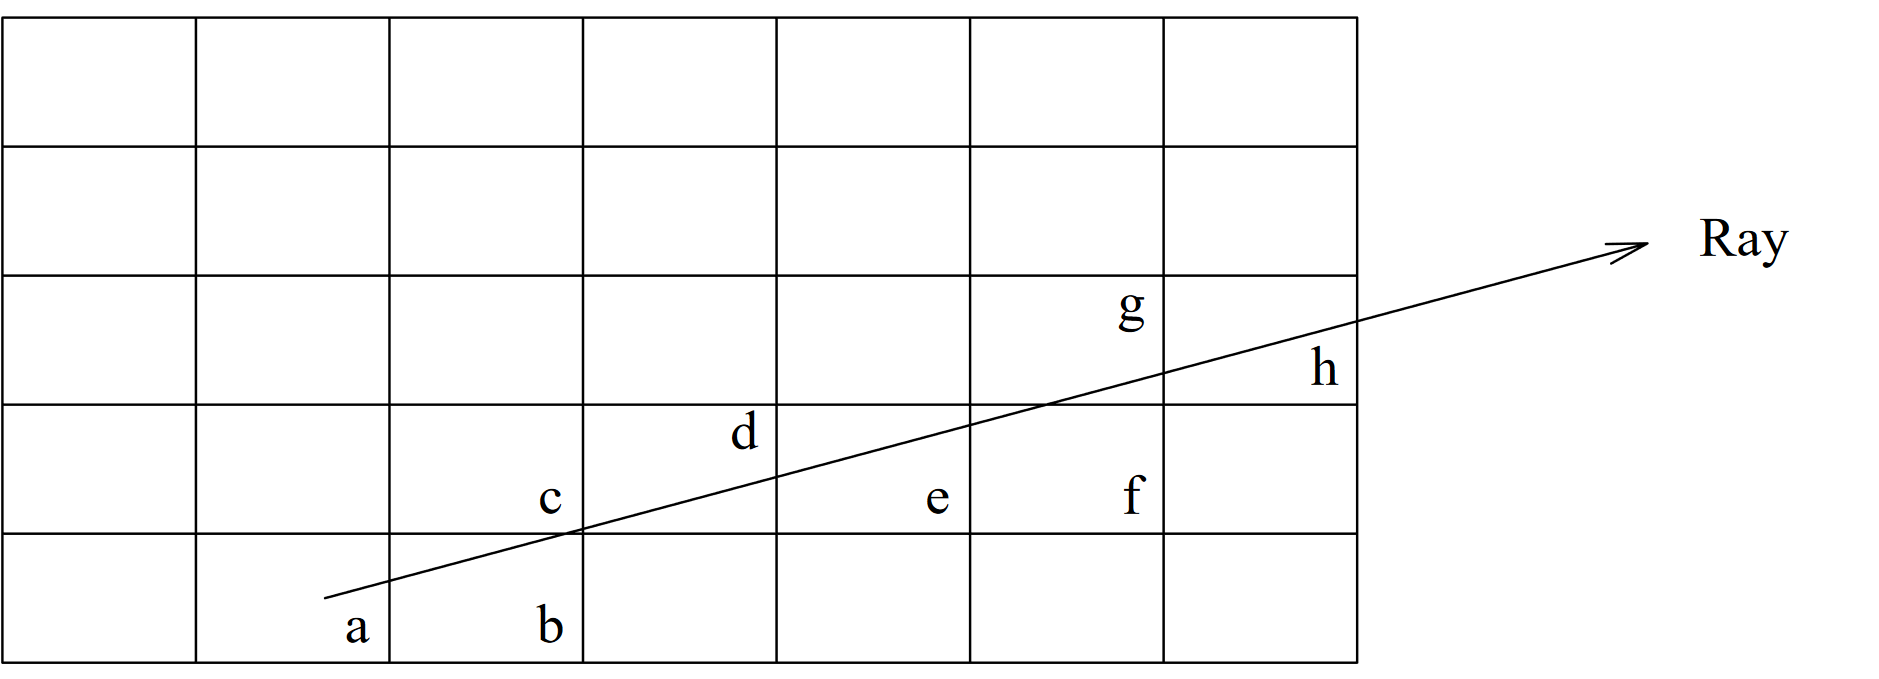
\includegraphics[width=\linewidth]{figures/dda.png}
    \caption{A ray being shot through a dense grid and marking every traversed voxel with a letter. \cite{amanatides1987fast}}
    \label{fig:dda_traversal}
\end{wrapfigure}

\subsection{Voxel data structures} \label{related_work:voxel_data_structures}
Data structures for volume data have seen multiple forms trying to optimize ray marching performance, memory footprint, update speed and simplicity. This research specifically targets heterogeneous volumes which often consist of gradients where outer voxels can have small non-zero values, instead of having opaque volume boundaries. We will briefly go over some major volume data structures, below.

\begin{wrapfigure}{r}{0.4\textwidth}
    \centering
    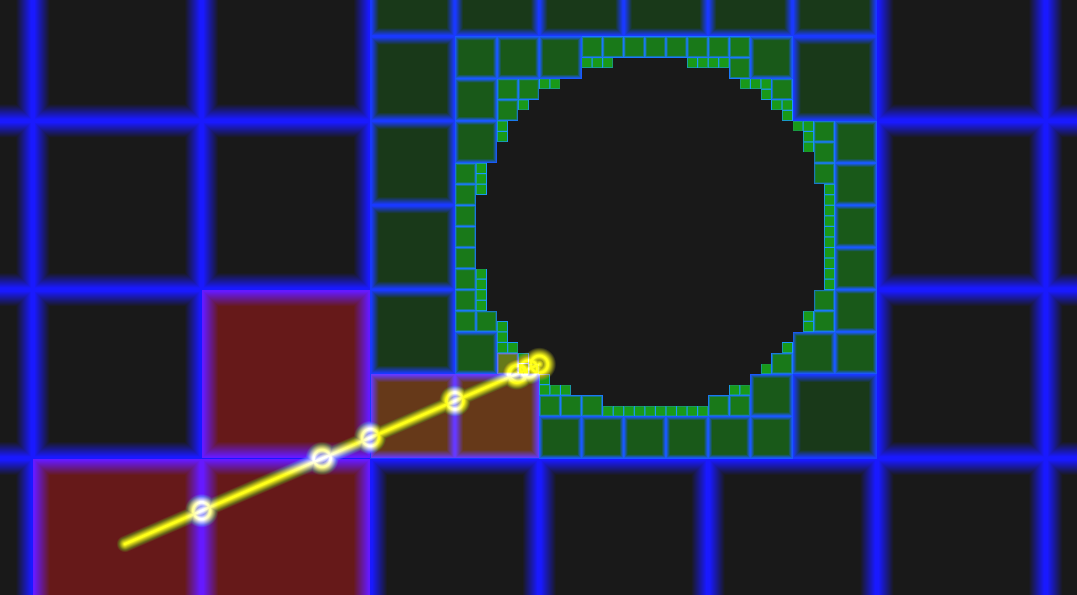
\includegraphics[width=\linewidth]{figures/esvo_traversal.png}
    \caption{Hierarchical digital differential analyzer (HDDA) traversal through a sparse voxel octree. The yellow line is our ray. The brighter green a cell is, the deeper our nodes in the octree are. We can see that nodes that are further away from the circle, can be stepped through with big steps, but as we approach the circle, our steps become smaller. \cite{ShaderToyQuadtree}}
    \label{fig:esvo}
\end{wrapfigure}




\subsubsection{Dense 3D grid} \label{related_work:voxel_data_structures:dense_grid}
The most basic structure (see Figure \ref{fig:dda_traversal}). Here, every value in the 3D array corresponds to a voxel. Indexing into this structure is fast and editing is trivial. However, there is no compression or space skipping. Another problem with flat arrays is their memory requirement as it has cubic scaling with the resolution. However, small-scale simulation software still often relies on this data structure as it is easy to implement, and in many cases, simulations have to update each voxel anyway.



\subsubsection{Efficient sparse voxel octrees (ESVO)} \label{related_work:voxel_data_structures:esvo}
A solution to the memory problems was proposed by NVIDIA, by introducing sparsity to homogeneous volume data \cite{laine2010efficient}. The main contribution is a data structure that drastically reduces the memory footprint by not storing information about homogeneous areas. This memory reduction also yields a speedup when traversing the volume, as larger steps can be taken through homogeneous areas (see Figure \ref{fig:esvo}). Along with that, the structure will more easily fit in the different caches of the GPU. However, due to the nature of tree structures, the data access pattern is less coherent which negatively impacts ray marching performance. The paper also did not take any form of animation into account. So this data structure only really works on static scenes \cite{JohnLinPerfectEngine}.


\subsubsection{Sparse voxel directed acyclic graphs} \label{related_work:voxel_data_structures:svdag}
A follow-up paper was released further improving the memory footprint optimization \cite{kampe2013high}. Here, the nodes of the octree can be reused for identical volumes, so one leaf can be the child of multiple nodes that share the same data (see Figure \ref{fig:DAG_node_deduplication}). The result is a significant reduction in memory usage over ESVO. Afterward, additional papers were written to, (1) further optimize the memory footprint by creating a lossy data structure which will slightly alter the volume data in an attempt to find more similar volumes \cite{van2020lossy} (LSVDAG). And (2) allow for real-time editing of this data structure \cite{careil2020interactively} (HashDAG).

\begin{figure}[H]
    \centering
    \subfloat[Removal of identical nodes in all levels of a binary tree. In the SVDAG paper, the same technique is applied to octrees. \cite{kampe2013high}]{
        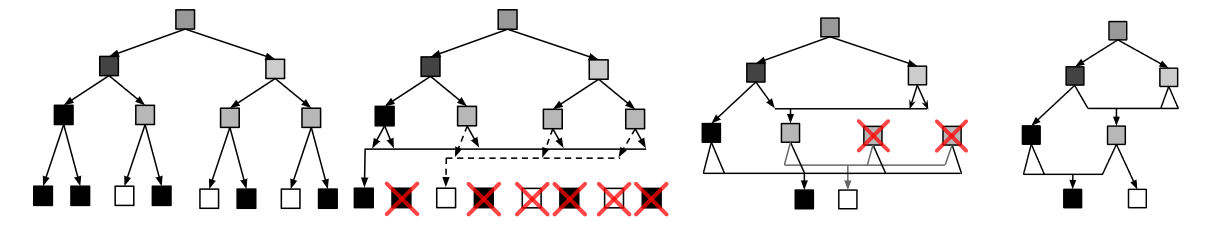
\includegraphics[width=0.45\textwidth]{figures/DAG_node_deduplication.png} \label{fig:DAG_node_deduplication}
    }
    \hfill
    \subfloat[Here we see the brick map (in red), which is dense. Whenever an area in this brick map is not homogeneous (indicated by the filled-in squares), we point to a brick (in blue). \cite{van2015real}]{
        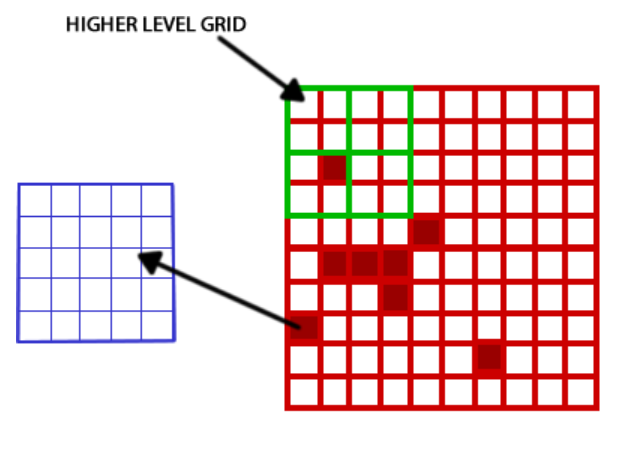
\includegraphics[width=0.45\textwidth]{figures/brickmap.png} \label{fig:brickmap}
    }
\end{figure}

\subsubsection{Brick map} \label{related_work:voxel_data_structures:brickmap}
Later another paper was released which tried to maintain part of the memory benefits from octrees while also improving ray marching performance \cite{van2015real}. This was done by keeping the idea of a hierarchical structure, but limiting the tree depth to 2 layers (a top-level grid, the brick map and the bottom-level bricks, as can be seen in Figure \ref{fig:brickmap}), which improves cache utilization. An additional benefit of reducing the depth of a data structure is the update time. When running a fluid simulation, which has to touch every leaf node in a tree, a shallower tree will take fewer steps when going down to the bottom of the tree to modify each voxel. Similar to the flat 3D array, the brick map structure is fast when it comes to update speeds, as both have shallow tree structures. Another paper explores implicit brick maps \cite{niessner2013real}. These are implicit because they don't encode their location in a grid, but hash a world position and use that hash to index into the brick buffer directly. This allows for an unbounded index space instead of having to create a grid inside a certain axis-aligned bounding box (AABB). However, nothing has been documented about them in the context of ray tracing.


\subsubsection{VDB} \label{related_work:voxel_data_structures:vdb}
In the movie industry, \textbf{VDB} \cite{museth2013vdb} has been the standard for volumetric rendering for a long time. This is a hierarchical B+tree structure with 3 layers (see Figure \ref{fig:VDB}), which optimizes for both query speed and memory size. It does so by making clever use of bit masks (see Section \ref{related_work:attribute_separation:bitmasks}), logical bitwise operations and inverted tree traversal. The last of these optimizations means that we don't have to traverse down the tree every time we query a point. But instead, we assume that consecutive points will be close to each other, and remember where we are in the tree. Then the next time we query a point we start at the bottom of the tree and have $O(1)$ access time if we retrieve a point that resides in the same bottom layer.

The VDB structure has mostly been used on the CPU. There have been implementations that port VDB to the GPU, but these do not support dynamic topology \cite{hoetzlein2016gvdb} \cite{museth2021nanovdb}. They would allow individual voxels to be modified, but can't place new voxels in arbitrary locations. This limitation makes simulation on the GPU impractical while maintaining the sparsity which makes the structure effective. The reason why this dynamic topology has never been implemented likely has to do with an inherent race condition when trying to modify any tree structure in parallel.

Research has also been conducted on encoding voxels or even internal layers of the VDB structure in neural networks \cite{kim2022neuralvdb}. These neural encodings can store a lot of detail in limited memory, but take minutes to train. Which, again, makes dynamic updates impossible.

One useful result of the standardization of VDB technology is the data format. Many tools can interface directly with the VDB file format \cite{VDBADeepDive}, and many artistic tools can export to the VDB file format. These features make it easy to download specific effects and test in a specific renderer.

\begin{wrapfigure}{r}{0.4\textwidth}
    \centering
    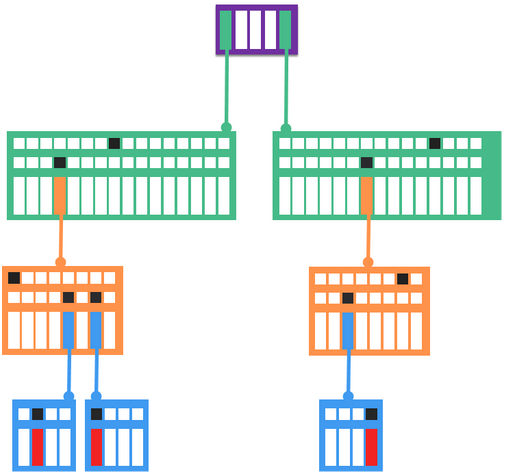
\includegraphics[width=\linewidth]{figures/OpenVDB.png}
    \caption{The four-level tree structure of the VDB data structure. In purple, we see the top node which has an arbitrary size and points to the first level of internal nodes. The two levels of internal nodes (in green and orange) both contain three rows of values. The top row is a bit mask indicating which values are "active" (this is application-specific), the middle row is a bit mask indicating that a child node exists, and the bottom row contains a pointer to the child node. Then in blue, we have a top row which is a bit mask indicating if a voxel is empty, and the bottom row containing the actual voxel data. \cite{museth2013vdb}}
    \vspace{-30pt}
    \label{fig:VDB}
\end{wrapfigure}




\subsection{Attribute separation} \label{related_work:attribute_separation}
All modern processors are built with cache hierarchies. These caches are usually a few megabytes and consist of many 128-byte cache lines. Which contain all recent memory accesses so, they can be reused quickly when the memory is fetched again. When accessing any memory, an entire cache line (of 128 bytes) is loaded. This means the memory access cost of fetching a single floating point value ($4$ bytes) is the same as fetching 32 ($128/4$) floating point values. Abusing this is key to writing fast CPU and GPU code. Therefore, it is crucial to have as little unused data within each cache line fetch as possible. This can be achieved by separating the voxel data from the geometry structure \cite{dado2016geometry}.
\subsubsection{Fast volume traversal} \label{related_work:attribute_separation:fast_volume_traversal}
There are two main branches of volume traversal. The first is by sampling the volume along a ray with certain step sizes. This is what delta tracking does (see Section \ref{related_work:path_traced_volume_rendering:delta_tracking}). Another method of traversing the volume is a more exact technique called digital differential analyzer (DDA) \cite{amanatides1987fast}. This analytically calculates how far along the ray we can step to arrive at the next voxel. Using this technique we also know exactly how much density we accumulated along our steps. This has benefits for the shading part of our render, but we won't go into that in this research. DDA has been extended to allow hierarchical volume data structures to be traversed, this is called a hierarchical digital differential analyzer (HDDA)\cite{laine2010efficient}.


Recently, NVIDIA has done research about using signed distance fields (SDF) to speed up traversal\cite{soderlund2022ray}. The general idea behind these distance fields is that the maximum step length a ray could take in any direction (without hitting anything) is pre-calculated, and used to skip over voxels that are known to be empty (see Figure \ref{fig:SDF_marching}). This method could be applied to most of the data structures described above, and might specifically be promising when combined with flat structures which don't implicitly store distance values by using bigger nodes in homogeneous volumes. However, calculating these SDFs is one additional step in the pipeline. Although this can be done quickly even for large volumes (less than $1$ ms for $1024^3$ voxels \cite{cao2010parallel}), it is unclear if the speedup during tracing outweighs the construction cost.
\subsubsection{Bit  masks} \label{related_work:attribute_separation:bitmasks}
When taking steps along a ray, there is a high chance that we will often access voxels that are close to each other, especially when using DDA, and we have to traverse all consecutive voxels. To reduce the bandwidth requirement of these methods we can use bit masks to indicate whether voxels are empty \cite{van2015real}\cite{museth2013vdb}. When using 32-bit floating point values as densities, for example, we can traverse all voxels that have a density of $0$ using the bit mask. Respectively, we can have a $16\times8\times8$ region of voxels in a single cache line, making our traversal significantly less bandwidth-heavy.

\begin{wrapfigure}{r}{0.4\textwidth}
    \centering
    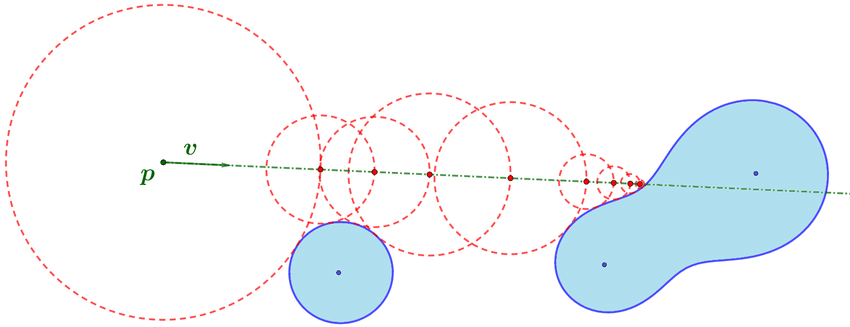
\includegraphics[width=0.9\linewidth]{figures/sdf_ray_marching.png}
    \caption{Marching through a signed distance field enables steps that are exactly as long, as the closest heterogeneity is far away. Here we see the ray in green, and the step sizes are indicated by the red circles. \cite{SDF_sphere_marching}}
    \label{fig:SDF_marching}
\end{wrapfigure}

\begin{table}[htbp]
    \centering
    \begin{adjustbox}{max width=\textwidth}
        \begin{tabularx}{\textwidth}{|c|X|X|X|X|X|}
            \hline
            \textbf{Method} & \textbf{Sampling Performance} & \textbf{DDA Performance} & \textbf{Memory Footprint} & \textbf{Update Speed} & \textbf{Simplicity} \\
            \hline
            Dense Grid      & \Plus \Plus                   & \Minus \Minus            & \Minus \Minus             & \Plus \Plus           & \Plus \Plus         \\
            \hline
            ESVO            & \Minus \Minus                 & \Plus                    & \Plus                     & \Minus \Minus         & \Minus              \\
            \hline
            SVDAG           & \Minus \Minus                 & \Plus                    & \Plus \Plus               & \Minus \Minus         & \Minus \Minus       \\
            \hline
            Brick map       & \Plus                         & \Plus \Plus              & \Minus                    & \Plus                 & \Plus               \\
            \hline
            VDB             & \Plus                         & \Plus \Plus              & \Plus                     & \Minus                & \Minus              \\
            \hline
        \end{tabularx}
    \end{adjustbox}
    \caption{An overview of the different data structures. The pluses and minuses provide some intuition into what every structure is optimized for. A very broad summary of the different metrics: The shallower the tree, the faster our sampling. Deeper trees have better DDA performance (see Section \ref{related_work:attribute_separation:fast_volume_traversal} for a very brief description), but we get optimal performance when our nodes approximate the size of our caches and cache lines. Deeper trees improve memory footprint and deduplication improves it even further. The shallower our tree, the faster and easier our updates. And simplicity depends on the method.}
    \label{tab:structure-comparison}
\end{table}

\subsection{Texture compression} \label{related_work:texture_compression}
Although it might sound odd, we could learn a thing or two from texture compression techniques. They are similar to our voxel data in the sense that both contain floating point arrays. The only two differences are that textures usually store color data and are two-dimensional, while our volume data contains densities and is three-dimensional. These floating point arrays that textures use have pretty much always been too big for computers, at least when no compression is applied. Usually, photos are compressed using a lossy technique like JPEG, and logos or other digital assets without too many gradients are compressed using PNG which is not lossy. These methods work fine when we care about compression ratios, but they do not when we want to do billions of texture fetches per second on the GPU. For this purpose block compression is usually being used\cite{BlockCompression}. Block compression has different formats for different use cases. For example, BC4 is suitable for grayscale textures, and BC5 is optimal for normals (as seen in Table \ref{tab:block_compression}). These formats all encode $4\times 4$ pixels into a certain number of bytes, which can be used for 2D textures but also technically work in three dimensions. However, we do get spatial dependencies in two out of three axes then, these are the dimensions in which the $4\times 4$ chunk is arranged.

\begin{table}[htbp]
    \centering
    \adjustbox{max width=\textwidth}{
        \begin{tabular}{|c|c|c|p{5cm}|}
            \hline
            \textbf{Type} & \textbf{Data Rate}         & \textbf{Palette Size} & \textbf{Use For}                     \\
            \hline
            BC1           & RGB + optional 1-bit alpha & 0.5 byte/px           & Color maps                           \\
                          &                            &                       & Cutout color maps (1-bit alpha)      \\
                          &                            &                       & Normal maps, if memory is tight      \\
            \hline
            BC2           & RGB + 4-bit alpha          & 1 byte/px             & n/a                                  \\
            \hline
            BC3           & RGBA                       & 1 byte/px             & Color maps with full alpha           \\
                          &                            &                       & Packing color and mono maps together \\
            \hline
            BC4           & Grayscale                  & 0.5 byte/px           & Height maps                          \\
                          &                            &                       & Gloss maps                           \\
                          &                            &                       & Font atlases                         \\
                          &                            &                       & Any grayscale image                  \\
            \hline
            BC5           & 2 $\times$ grayscale       & 1 byte/px             & Tangent-space normal maps            \\
            \hline
            BC6           & RGB, floating-point        & 1 byte/px             & HDR images                           \\
                          &                            &                       &                                      \\
            \hline
            BC7           & RGB or RGBA                & 1 byte/px             & High-quality color maps              \\
                          &                            &                       & Color maps with full alpha           \\
            \hline
        \end{tabular}
    }
    \caption{Block compression formats and use cases \cite{BlockCompression}.}
    \label{tab:block_compression}
\end{table}




\subsection{Gaps in current research} \label{related_work:gaps_in_current_research}
There are of course still many issues with volume data structures, so below are some of the most notable issues with the current state-of-the-art, and how we can push the state-of-the-art forward in a meaningful way. Many methods have either optimized volume data structures for memory usage \cite{laine2010efficient}\cite{kampe2013high}, ray tracing performance \cite{van2015real} \cite{soderlund2022ray} \cite{museth2013vdb} or simulation times (flat 3D array). However, none of these techniques currently can do all three of these things while keeping all data and computation on the GPU. Below are two issues that this research tries to address.
\subsubsection{Large assets} \label{related_work:gaps_in_current_research:large_assets}
Video game assets have been growing in size to the point where games can be hundreds of gigabytes. Adding another asset type, volumes would further increase this. So although there has been a lot of research done in compressing geometry (the volume shape without its per voxel attributes) to the point where entire scenes can be voxelized into game-ready asset sizes\cite{van2015real}\cite{museth2013vdb}. We also need our actual density data to be small, which has been done by \cite{dado2016geometry}, but this was applied to normals and colors, not specifically densities which only have one floating point value per voxel instead of three.
\subsubsection{Animation delta compression} \label{related_work:gaps_in_current_research:animation_delta_compression}
Another thing that has not been explored extensively is applying delta compression on our volumes. This has been hinted at by \cite{careil2020interactively}, where they suggest encoding animation frames as different branches of the tree. Resulting in a structure that can simply swap some pointers at certain points in the tree when changing to the next frame. However, there are two issues with this method: (1) The deep quad-tree structure is not optimized for tracing, and when flattening the structure we rapidly reduce the effectiveness of deduplicating our nodes. (2) This does not change the attributes of the lower-level nodes, so when our attributes change (a density increases or decreases) we would have to swap pointers high up in the tree, effectively requiring a new tree for every animation frame.
\clearpage
\section{Requirements} \label{requirements}
\subsection{Asset size} \label{requirements:asset_size}
\subsection{Sampling speed} \label{requirements:sampling_speed}
\subsection{Animation playback} \label{requirements:animation_playback}
\subsection{Lossy compression} \label{requirements:lossy_compression}
\subsection{Level of detail} \label{requirements:level_of_detail}
%This section is split up into two parts, namely functional and non functional requirements. The former describes certain functionalities which the program should have, and the latter describes how it does said things and how well it does said things. Below, the functional and non functional requirements are listed along with a description and reasoning of each requirement.
%
%\subsection{Functional Requirements (FR)}\label{requirements:FR}
%\begin{enumerate}
%    \item \textbf{The data structure needs to be traversable by \href{https://traverseresearch.nl/}{Traverse}'s rendering framework on the GPU.} To make the project useful for \href{https://traverseresearch.nl/}{Traverse} (and to make implementation easier), the project needs to be written in the existing Breda framework. This will require adhering to everything which was discussed in Section \ref{introduction:traverse}. However, when benchmarking against the current state of the art (NanoVDB\cite{museth2021nanovdb}) it will be too time consuming to implement entirely in \href{https://traverseresearch.nl/}{Traverse}'s framework. So NanoVDB will be evaluated in Cuda/c++. \label{FR:framework}
%    \item \textbf{Every cell in the data structure must be able to hold a certain set of values.} For our volumetric data structure to be useful it somehow needs to store data about its volume. This can be the density of particles, the material that is being traversed or the brightness of light emission. For example, if we traverse a cloud we only really care about the density, but when traversing an explosion we also care about the light emitted by the fire. So there needs to be a way to have the leaves of our data structure contain arbitrary data (with a known size at compile time), while not impacting the ray marching performance. Note that it is enough for every voxel to have the same number of properties, there is no need for a varying number of properties within one volume. Making sure the performance stays roughly the same with an increase in the number of properties, can be done by using bitfields for intersection testing and only once an intersection has been found, we use a pointer to go to the actual data of our leaf node. This way the efficiency of caching wont degrade as our leafs get more attributes. \label{FR:datalayout}
%    \item \textbf{The data needs to retain the resolution it was imported from.} It is important that we optimize the ray tracing performance while retaining the original resolution. Not only might there be issues regarding the expected visuals and the actual visuals if we start altering the amount of detail. But we can also run into graphical artifacts.
%          As described in \ref{introduction:voxel_data_structures}, we might be able to speed up the rendering process by getting the max and min density values in a certain area as close to each other as possible. So it might be worth investigating if this can be done, and if the benefits in performance outweigh the reduction in quality. \label{FR:resolution}
%    \item \textbf{Interface with OpenVDB\cite{museth2013vdb}, the industry standard for volumetric data exchange.} This is the go-to method for generating/storing/distributing volumetric data and thus very important if we want to interface with tools like Houdini\cite{Houdini}. We need to be able to read the VDB files from disk, then store that data in a VDB data structure in RAM, and then transform that into our final data structure. The VDB portion of this pipeline already exists. We just need to create a transform to our desired data structure. \label{FR:interfacing}
%    \item \textbf{Animation needs to be possible without copying volume data back and forth from the GPU.} In general, syncing data from the GPU to the CPU can be a major cause of idling as the CPU waits for the data to be transferred. Another issue has to do with syncing the data. Lets say there is a simulation running on the GPU, but the CPU retrieved the volume data to modify it in some way. Now once the CPU uploads its data back to the GPU, it will overwrite anything the GPU just did. So not only is this copying of data a performance but also a programming problem. In this case animation includes at least a simple fluid or particle system, along with the built in animation for OpenVDB. \label{FR:animation}
%\end{enumerate}
%
%
%
%
%
%\subsection{Non-functional requirements (NFR)}\label{requirements:NFR}
%\begin{enumerate}
%    \item \textbf{The most important part of this research, is to test the viability of animation.} For clouds, it might be possible to use static volumes. But for almost anything related to physics, we need the structure to be dynamic. Explosions, fire or dust storms require animation and thus the volume data needs to be efficiently editable. This means that not only do we need the values within each voxel to be changed, but the entire structure of our volume needs to be able to change. When using a sparse data structure, new nodes must be allocated during the simulation as we need them. As a guideline we are aiming to reliably update 100k voxels every frame, while not sacrificing the sparsity of the used data structure.\label{NFR:update}
%    \item \textbf{Secondary is the ray tracing performance.} Traverse Research is a real time graphics company. So everything they do has to, at some point, fit into a few milliseconds per frame. Given that volumes can have a resolution of $16^3$ to $1024^3+$ voxels and there can be millions of rays entering the volume every frame, we need a way to speed up the process of traversing. Some research has already been done in this area, as described in Section\ref{introduction:volume_acceleration}. This is not the most important part of the project as the optimization process of ray tracing techniques can become very open ended. Along with that, adding animation to the existing GPU data structures would push volumetric data structure research forward in a more significant way. \label{NFR:tracing}
%    \item \textbf{Third is the memory footprint.} Memory footprint is often tied to ray tracing performance due to caches, but not necessarily. In modern engines, the GPU needs to keep many different resources in memory. These are resources like acceleration structures, textures and buffers. So to keep the solution viable in a large game engine, we need a small data structure. \label{NFR:memory}
%    \item \textbf{Lastly, the data needs to be sparse to reduce the memory footprint of homogeneous areas in given volumes.} Although this is closely tied to NFR \ref{NFR:tracing} and NFR\ref{NFR:memory}, we wanted to emphasize the necessity of sparsity. This sparsity will allow the performance to scale up and down depending on scene complexity. It would be wasteful if a tiny cloud in a large volume would require the same amount of memory as a cloud which would fill the entire volume. \label{NFR:sparsity}
%\end{enumerate}
%
%\subsection{Concretization}\label{requirements:concretization}
%These requirements lead us to the main goal of this research, a sparse dynamic hierarchical data structure for volumes. Now we do run into an issue with the definition of animation, as we want to support both simulation and playback of VDB animations. When we focus on simulation, we need a shallow tree which can quickly allocate all required nodes. Preferably, able to simulate millions of particles and insert all of these quickly into our data structure. When we want a data structure for animation, we have to focus on data size. We can, for example, store each animation frame into separate trees. But  we quickly run into memory issues this way, so we need to somehow re-use information from our tree across frames. This will be done using a similar algorithm for node de-duplication as described in the SVDAG paper \cite{kampe2013high}. Fortunately we can take as long as we want for this pre-processing step. Now both of these solutions will result in sparse trees which will be traversable on the GPU, and have the same architecture as VDB. We will use a dynamic top node, then at least one internal layer of nodes, and then the leaves which contain the highest resolution data. Furthermore, we will make use of bitmasks to quickly check the existence of child nodes, and support arbitrary data in the internal nodes to support LOD's and local min/max data.
\clearpage
\section{Research questions}\label{research_questions}
Resulting from our introduction and requirements there are two main questions that we want answered which are written below.

\subsection{Optimal data structure}\label{research_questions:optimal_data_structure}

\noindent\textbf{What data structures, or combination of structures, are optimal for ray tracing, memory and animation, and can these structures be converted into each other?} We have already seen that there are different techniques which are optimized for different metrics. So if we know the optimal method for each of our requirements, we can work towards combining their strengths without having to create one structure which can do it all (which evidently does not exist, yet).

\subsection{Performance bottlnecks}\label{research_questions:performance_bottlenecks}
\noindent\textbf{Is volume traversal memory or compute bound?} This question should provide insight into future optimization techniques. Insight into questions like "if L1 cache size is increased by X amount, will this improve volume traversal speed?" or "if the clock speed of a GPU is increased, what will the impact on our volume traversal be?" will be acquired.

\clearpage
\section{Approach} \label{approach}
In this section we describe how we went about the creation of our data structure and what the different considerations were. This includes the high level ideas which resulted in our data structure.
\subsection{VDB data structure} \label{approach:vdb_data_structure}
The data structure of choice is VDB. This is a compromise between ray tracing performance and compression, and can be extended or reshaped (internal layers could be removed, added or changed in size) if desired. However, the top level node, which can be indefinitely large, was not used. This removes the need to perform the expansive hash table step, and also removes the need for our accessor types. Additionally, this restricts our index space to a certain region. In our implementation we chose the standard 5-4-3 VDB layout resulting in an index space of $1 << (5+4+3) = 4096$ cubed. More than large enough for most VDB files. This has a few implications: a completely empty volume uses $((1<<5)^3+((1<<5+4)^3)) / 8 = 16$MB, because we always allocate 1 top level node along with one 2nd level node for every bit in the top level node's bitmask. There are also always 3 indirections before we can access our voxel data. And our large higher level nodes will rarely contain duplicates (as required for a technique as described in Section \ref{related_work:voxel_data_structures:svdag}).

\subsection{Simulation} \label{approach:simulation}
As part of implementing a dynamic VDB data structure there was some work done regarding a GPU modifiable version. Unfortunately due to time constraints this was never fully implemented nor tested. However, there were some findings about how such a system could be implemented.

Modifying a sparse volume data structure on the GPU has many inherent issues. One of those issues arises because the GPU is a massively parallel system which requires cautious handling of synchronization. When implementing a VDB-like structure with 3 indirections (top level node, 2 internal layers, and the voxel data) we have to make sure that all parent nodes are present. One way of doing this would be to check if the parent exists, if not, we create it. We can create the parent node by keeping track of an atomic counter which is used for indexing into a large buffer in which we allocate our parent. However, what if we allocate two voxels with the same parent, then we will allocate twice and have that the parents parent point to one of the allocated nodes. This is a race condition.

Let's say we tried to use that scheme, but we use one of the essential parts of the VDB data structure, the bitmask. So we use an atomic bitwise or operation on the bitmask which sets the correct bit to true. This operation will also return the original output, which for one thread will be false, and for all other threads which did the atomic operation, will be true. So now we have a single thread which can allocate the node and set the parents parent pointer right? Well no, the GPU can, at any time, swap out the currently running warp. So there is the possibility for one warp to set the bit, and be responsible for setting the parents parent pointer, but it being swapped out. This would result in other threads assuming that the pointer is already set, and them accessing garbage data.

So the only real way to handle this situation is to set the bits and pointers without reading either of these values within the same dispatch. This necessitates the separation of the initialization of the different layers of the tree into different dispatches. However, this does raise a new problem, how do we know which top level nodes to allocate and which bits to set. We could iterate over our entire dataset for every dispatch to find which nodes have to be allocated, but this might be wasteful if our dataset is large.

To conclude, if an editable VDB data structure is desired, it can be done. However, it will necessitate the use of at least 3 dispatches which might all need to access the entire dataset. If the dataset is not too big this might be fine because of the GPU's high bandwidth.

\subsection{Flip book animations} \label{approach:flipbook_animations}
Flip book animations are the opposite of delta compression. It means that we store every frame as a separate data structure, disregarding any temporal coherency. So why mention them, when they are not what we need. If we look at the actual data being used we see that by far the largest amount of memory is being used by the actual voxel data. Depending on what tree structure we use, this can be a larger or smaller part of our structure. Which leads to another interesting observation. If all these data structures use voxels as their leaf values, they could all share these leaf values. We can build different structures on top of a set of voxel bricks. For example, we can have a set of bricks in a brickmap to run a simulation, then mesh these bricks, so we can use the hardware rasterizer to find primary intersections. After which we can traverse them using DDA (see Section \ref{related_work:attribute_separation:fast_volume_traversal}) and do our shading. All these operations utilize the same underlying voxel data. So if we can get that as small as possible, we should be able to use an appropriate 'interface' to our data and have exactly what we need. Whether this is a flat or deep tree, or even something like a triangle mesh or BVH. This is why we mostly look at compressing our voxel brick data as much as possible. For animations, we have thus decided to use a simple flip book animation for the tree, while using one large voxel brick buffer.
\subsection{Texture compression} \label{approach:texture_compression}
Keeping our voxel brick data in a large buffer can only do so much on the GPU. We are bound by 32bit loads, have to set up a cache friendly access structure ourselves, and most importantly, can not use block compression. This is why the voxel data is stored in a sampled 3D texture. Using this texture we automatically get optimized access to our voxel data in the same way that 2D textures have fast access for filtering. The actual bricks should now be stored in texture slices, so we can create a texture with a certain width, height and depth (divisible by 8, our brick size). Then use some clever indexing to have a single unsigned integer point to a place inside this brick texture.


To compress our data there are a few new possibilities. Because we can skip these 32bit loads, we can easily store 16 bit floating point or unsigned normalized values (8 bit floating point values between 0 and 1). These normalized values can de denormalized to get the original values back. So now we have an easy way of reducing our voxel data by $4\times$. But we can go even further. BC4 (See Section \ref{related_work:texture_compression}) is a block compression method made for grayscale values, perfect for our density values. It encodes grayscale values at $0.5$ byte/pixel, meaning that we can store two voxels per byte. This already shrinks our data from 32bit per voxel to 4bits, an eight times reduction. However, we can use one last optimization using block compression. If we recall how block compression works, we see that it somehow compresses $4\times 4$ pixels. Now if we use one of the block compression techniques which encodes full RGBA data we get four floating point numbers per pixel, resulting in $4 \times 4 \times 4$ values. We can exploit this by storing our voxel data as separate color channels in our texture. When using either BC7 or BC3 we can encode floating point values at 1 byte/pixel. However, each of our pixels contains four density values, thus shrinking our volume data even further to a rate of 2bits per voxel. This is a sixteen times reduction over using full 32bit floating point values.

\subsection{Clustering similar nodes} \label{approach:clustering_similar_nodes}
One of the most fundamental techniques when compressing data is the reduction of duplicates. But when using volume data, or any floating point data, there is a low chance of having exact duplicate data. But when looking at large volume datasets there is a decent chance that two bricks will have roughly the same data. This can be the almost homogeneous inside a cloud, or a non-moving part of an animation for example. We can identify these similar bricks using clustering. This idea was inspired by \cite{van2020lossy} where they performed clustering on the voxel geometry. However unlike that technique, we specifically want our density data to be compressed. So we perform k-means clustering using a naive per voxel distance metric. However, there are two issues with this which can be worked around. (1) low density bricks will always be similar, and (2) bricks which are similar for almost all density values except for a few, we get a high similarity, yet we lose a lot of important detail. Both of these issues can be negated by introducing a variance threshold. We normalize all density values inside a brick, and then calculate the variance of all values in the brick. If this is above some set threshold we simply do not include it in our clustering, and keep using the original value. This way we do lose the ability to cluster smooth gradients, but we do make sure that we keep as much detail as we want.
\clearpage
\section{Implementation} \label{implementation}
Below are the different components that have been implemented to support this research. The entire implementation exists inside the Breda repository and is written in Rust and HLSL, this is why all code samples also use these languages.

\begin{wrapfigure}{r}{0.5\textwidth}
    \centering
    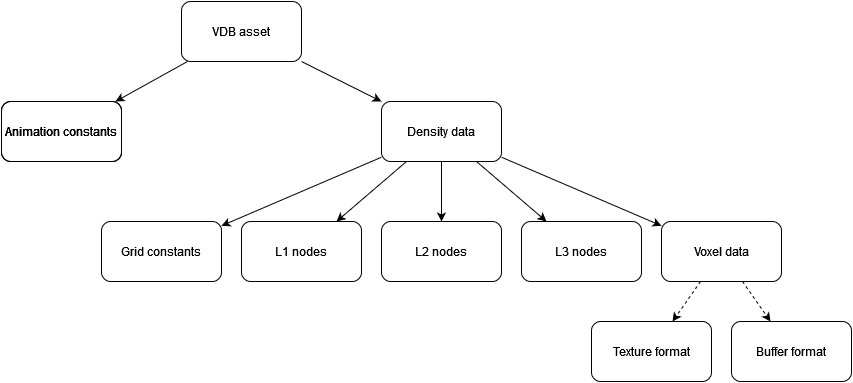
\includegraphics[width=\linewidth]{figures/vdb_asset.png}
    \caption{VDB asset data structure. Each VDB asset has constants for the entire animation, and density data. This density data has all the constants, nodes and voxel data. This voxel data can either be in buffer or texture layout. }
    \label{fig:vdb_asset}
\end{wrapfigure}

\subsection{Asset pipeline} \label{implementation:asset_pipeline}
The Breda asset pipeline is used to load all VDB files. This allows us to specify how our assets are loaded and processed, along with caching our final assets to reduce the amount of rebuilding. The main tweakable options for our VDB asset processing pipeline are the format, grid, filenames and clustering options. The format can be any of 32bit floating point, 16bit floating point, unsigned normalized (8bit float between 0 and 1) and BC7 \ref{related_work:texture_compression}. The grid specifies which grid in the VDB file we use as our density data. Usually, there are multiple grids in each VDB file, we can have density, temperature and volume type for example. All of these grids are used for different parts in a rendering pipeline, but for this research, we are only interested in a single grid and that is the density grid. The filenames option is used to select one or multiple VDB files, when entering multiple filenames we assume that these are an animation sequence. The clustering options consist of three things: (1) the number of clusters, which is $k$ when running k-means. (2) The number of iterations of k-means. And (3) the variance rejection threshold, which is used to specify how heterogeneous our bricks can be before we stop clustering them.

\begin{figure}[H]
    \centering
    
\includegraphics[width=\linewidth]{figures/voxel_memory_view.png}
    \caption{Voxel data texture captured by the Nsight frame debugger. Tiles of $8\times 8$ pixels can be seen. The third dimension, to get our brick data, is encoded using the RGBA color channels and the next texture slice. The tiles often contain gray values, meaning that the voxels in the z-axis are roughly the same (a pixel with roughly similar color values will always be a grayscale). However, some pixels are more colorful, which means that not all color channels are the same and there is either one voxel in the z-axis which is significantly different, or there is a gradient. This slice of the voxel brick data also showcases that even on this small scale of the individual brick level, there are many high-frequency details.}
    \label{fig:vdb_asset:memory_view}
\end{figure}


Using these options we can compute our VDB asset (The entire pipeline can be seen in Figure \ref{fig:vdb_asset_pipeline}). This consists mostly of constants and GPU-friendly vectors of data (see Figure \ref{fig:vdb_asset}). All nodes are implemented as structs which contain an unsigned integer to point to the next level of nodes and an array that contains unsigned integers. These are interpreted as the active child bit masks. In code, we refer to the internal nodes as L1, L2 and L3 nodes. L1 being the top level node with size $(1 << 5)^3$, L2 having size $(1 << 4)^3$ and L3 having size $(1 << 3)^3$ and pointing into the voxel data. The different animation frames are all unique L1 nodes. So if we want to render a specific frame we can simply take the frame ID and use that to index into the L1 nodes buffer, all pointers after that are handled at the asset creation stage. The full VDB asset creation process is listed below and with an overview in figure \ref{fig:vdb_asset_pipeline}.
\begin{enumerate}
    \itemsep0em
    \item First we read the metadata of our VDB files, which we then use to select which grid we want to read.
    \item Now we load the VDB data using vdb-rs \cite{VDBRS} which was developed during this research.
    \item Then we transform this data into our flat GPU-friendly data.
    \item The first pre-processing step consists of our deduplication scheme described in Section \ref{approach:clustering_similar_nodes}.
    \item After this we transform our data layout from our easy (and locally coherent) buffer layout to the texture layout.
    \item Then, depending on which format options were used, we compress our data. So we reduce our floating point data to either 16bit, 8bit or Bc7 texture data.
    \item After which we upload everything to the GPU.
\end{enumerate}

\begin{figure}[H]
    \centering
    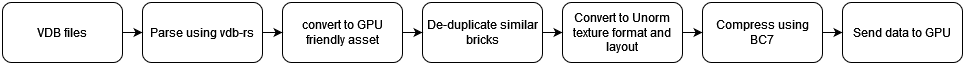
\includegraphics[width=0.9\linewidth]{figures/VDB asset pipeline.png}
    \caption{An overview of the asset creation pipeline.}
    \label{fig:vdb_asset_pipeline}
\end{figure}


\subsection{Shaders} \label{implementation:shaders}
To integrate the built data structure into Breda, two shaders have been written, \textit{VDB.hsls} and \textit{HDDA.hlsl}. The main way to interface with the data structure is contained in \textit{VDB.hlsl} which has functionality for getting voxels, getting the activity status of certain voxels, and checking what the deepest level of the tree a certain voxel is part of. \textit{HDDA.hlsl} is largely the same as implemented by \cite{museth2013vdb}. The main difference is that we make use of callbacks on the GPU, which is done by passing a template argument to the traversal function. This template argument must implement \textit{empty} and \textit{operator()} which are called after every step, or compiled away if either of them is not used. These step functions are used to write clean yet fast traversal code (as seen in Figure \ref{implementation:hdda_sample}).


\begin{figure}
    \begin{lstlisting}
    // The hdda march method has the following function signature
    // We explicitly say which level of our tree we want to traverse
    template <typename VoxelData, typename VoxelFn>
    void march(inout VoxelFn fn, Layer callbackLayer);

    // We define a struct that contains our traversal payload
    struct FirstDensityFn {
        float4 color;
    
        bool operator()(float voxelData, float t0, float t1, uint dataIndex) {
            float chunkIndex = voxelData * 360;
            color = float4(hsvToRgb(chunkIndex, 1, 1), 1);
            return false; // we do not want to continue traversal
        }
        bool empty(float t0, float t1, uint dataIndex) { 
            return true; // we continue traversal
        }
    };

    // Now we can simply perform our HDDA traversal as follows
    float4 traverseVolume(){
        Hdda hdda = Hdda::new_(volumeGrid, ray, inverseRay);
        FirstDensityFn fn;
        fn.color = float4(0,0,0,0);
        hdda.march<float>(fn, LayerVoxels); 
        return fn.color;
    }
\end{lstlisting}
    \caption{Simplified outline of the HDDA api.}\label{implementation:hdda_sample}
\end{figure}


\subsection{Compression} \label{implementation:compression}
As said in Sections \ref{approach:texture_compression} and \ref{approach:clustering_similar_nodes}, there are two types of compression of the voxel data going on. First, we will have a look at how to cluster similar bricks. This is largely done by using NDarray \cite{NDarray} for different linear algebra methods. The clustering process is divided up into the following steps:

\begin{enumerate}
    \itemsep0em
    \item We parse our voxel data into a 2D matrix where every brick is one row, allowing us to use per-row clustering algorithms.
    \item Then we calculate the variance of the density data of each brick and divide that by the brick's mean density to get a normalized variance.
    \item We reject the brick if the normalized variance is higher than our set threshold. This way we only keep bricks that have low variance and thus have a low likelihood of containing unique features (see Section \ref{approach:clustering_similar_nodes} for the reasoning behind this step).
    \item After which we run k-means on all low variance bricks, with a given $k$ and the number of iterations. Unfortunately, this can be an expansive step as k-means has an algorithmic complexity of $O(nk)$ where n is the number of bricks in this case, and $k$ is the number of requested new bricks. So when both are large this step will become unpractical. However, most of the low variance bricks can be represented by a few new bricks, so $k$ should not be large anyway.
    \item After we have a new set of bricks we just have to fix the pointers of our L3 nodes and merge the filtered high variance bricks with the new bricks, and we are done.
    \item In figure \ref{fig:implementation:compression:cluster} we see the results of this compression technique.
\end{enumerate}


\noindent Texture block compression is done after rearranging the data from a buffer layout to a texture layout. With this data layout we can reduce the floating point precision, or even use the existing intel texture compressor \cite{ISPCTextureCompressor} to encode our data into Bc7. After doing this we still have to tell our backend what the format is of our texture, and then we are done. We can reuse our HLSL code for all formats because HLSL automatically samples different floating point types correctly.




\subsection{VDB viewer} \label{implementation:vdb_viewer}
A prototyping application was created for visualizing VDB files. This application can be used to load a single VDB file and display multiple debug views of the model as can be seen in Figure \ref{implementation:vdb_viewer:debug_views}. This application also allows quick testing of compression schemes as it bypasses the standard asset pipeline system that was discussed in Section \ref{implementation:asset_pipeline}.

\begin{figure}[H]
    \centering
    \subfloat[Shaded by accumulating density along the primary ray. The body of the cloud is hollow as can be seen.]{
        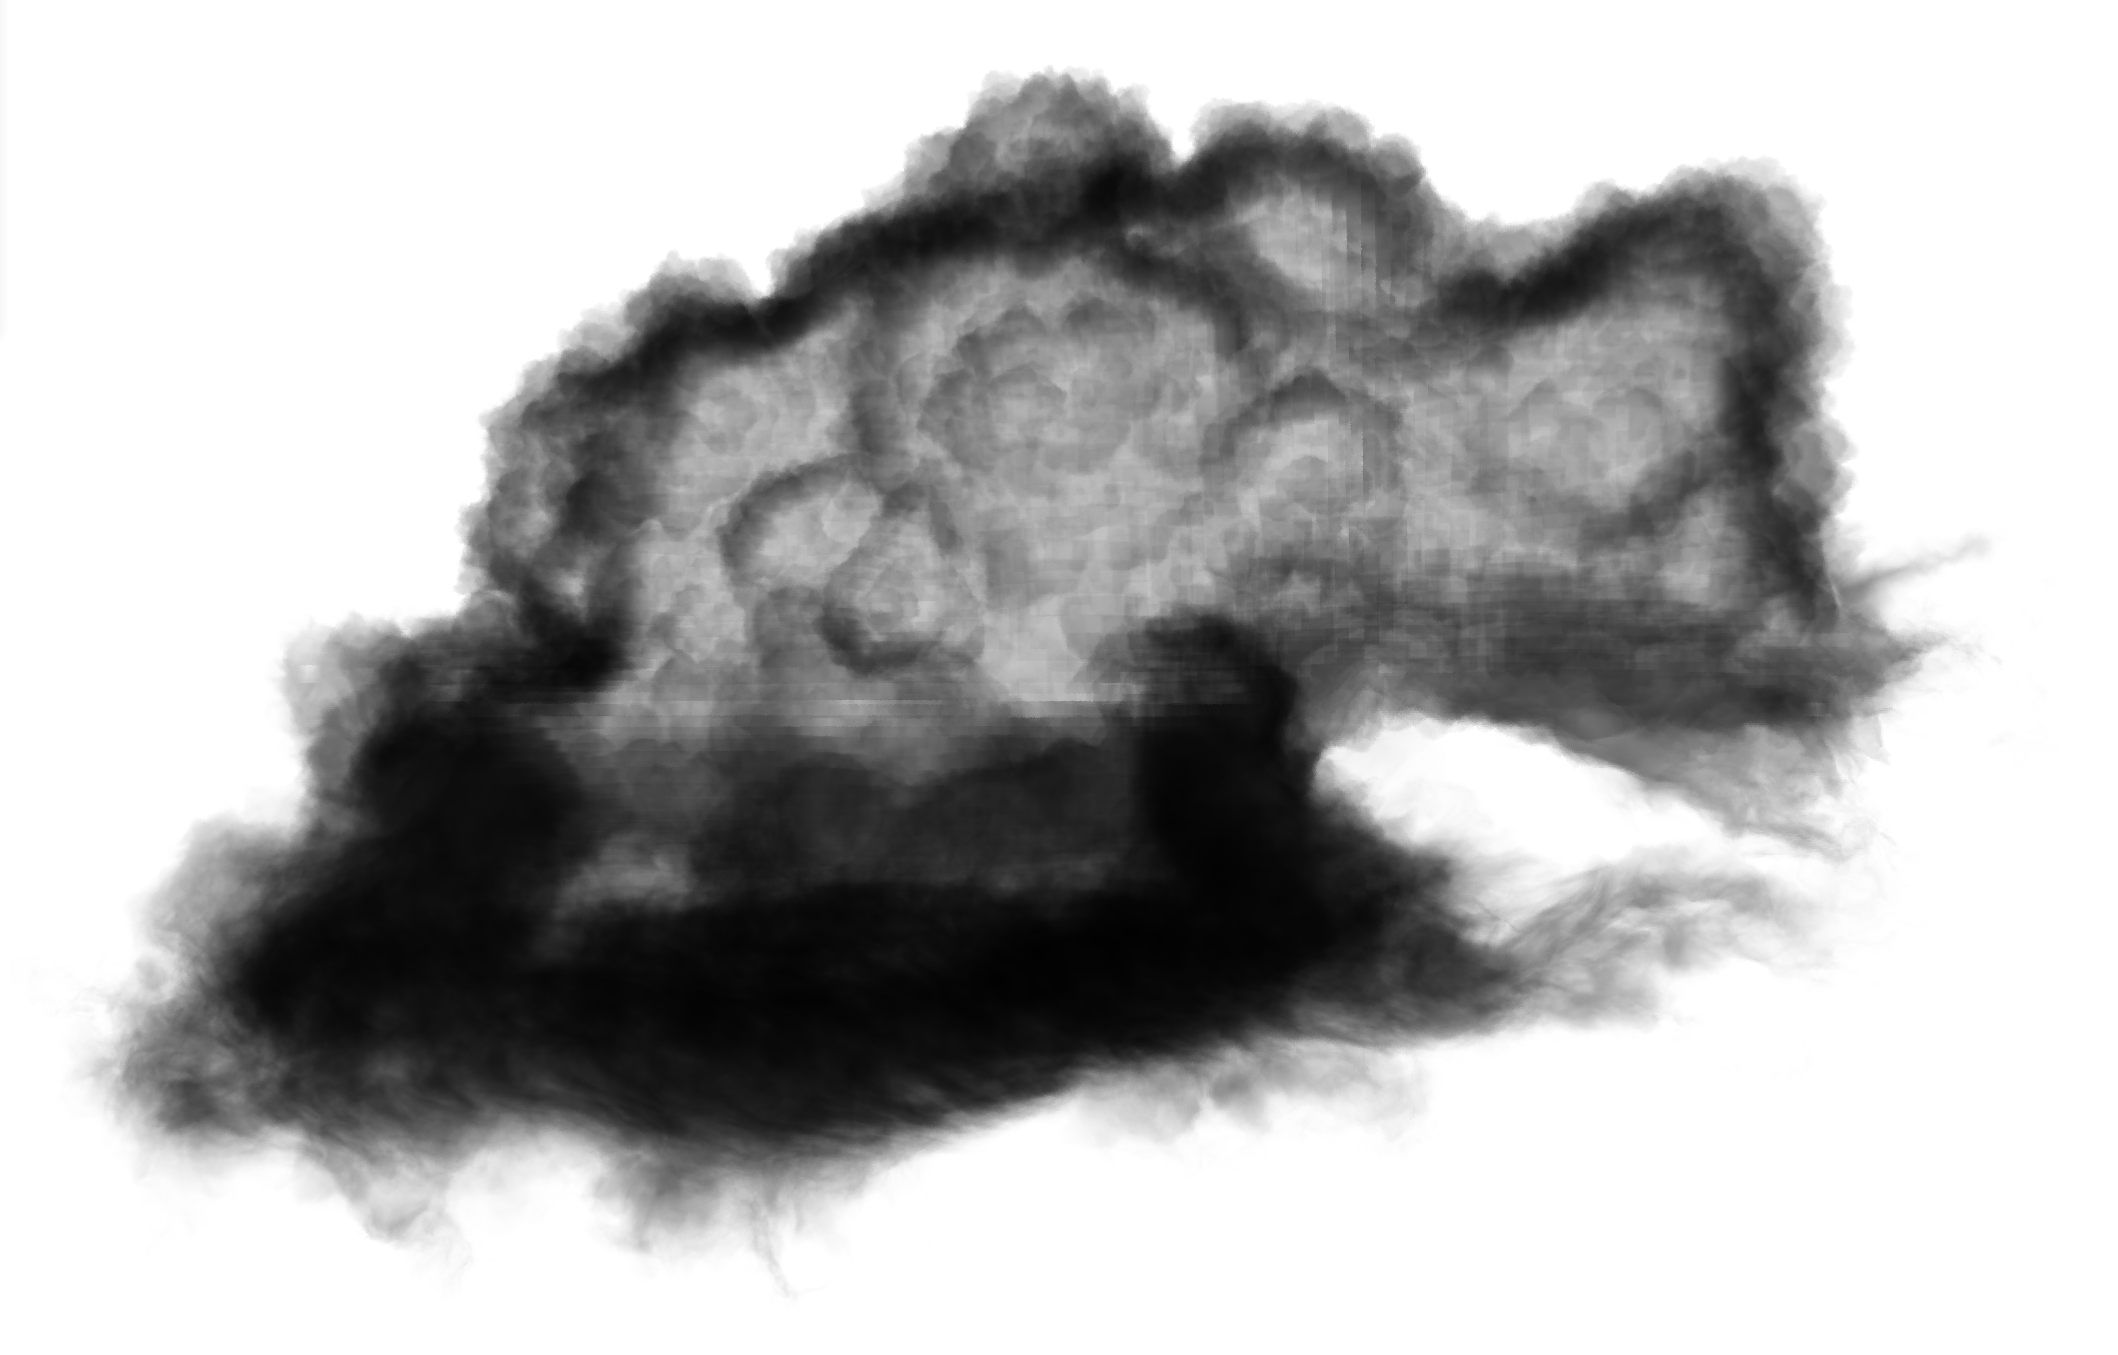
\includegraphics[width=0.45\textwidth]{figures/disney_cloud_half_res_shaded.png}
    }
    \hfill
    \subfloat[Shaded by depth of first hit voxel.]{
        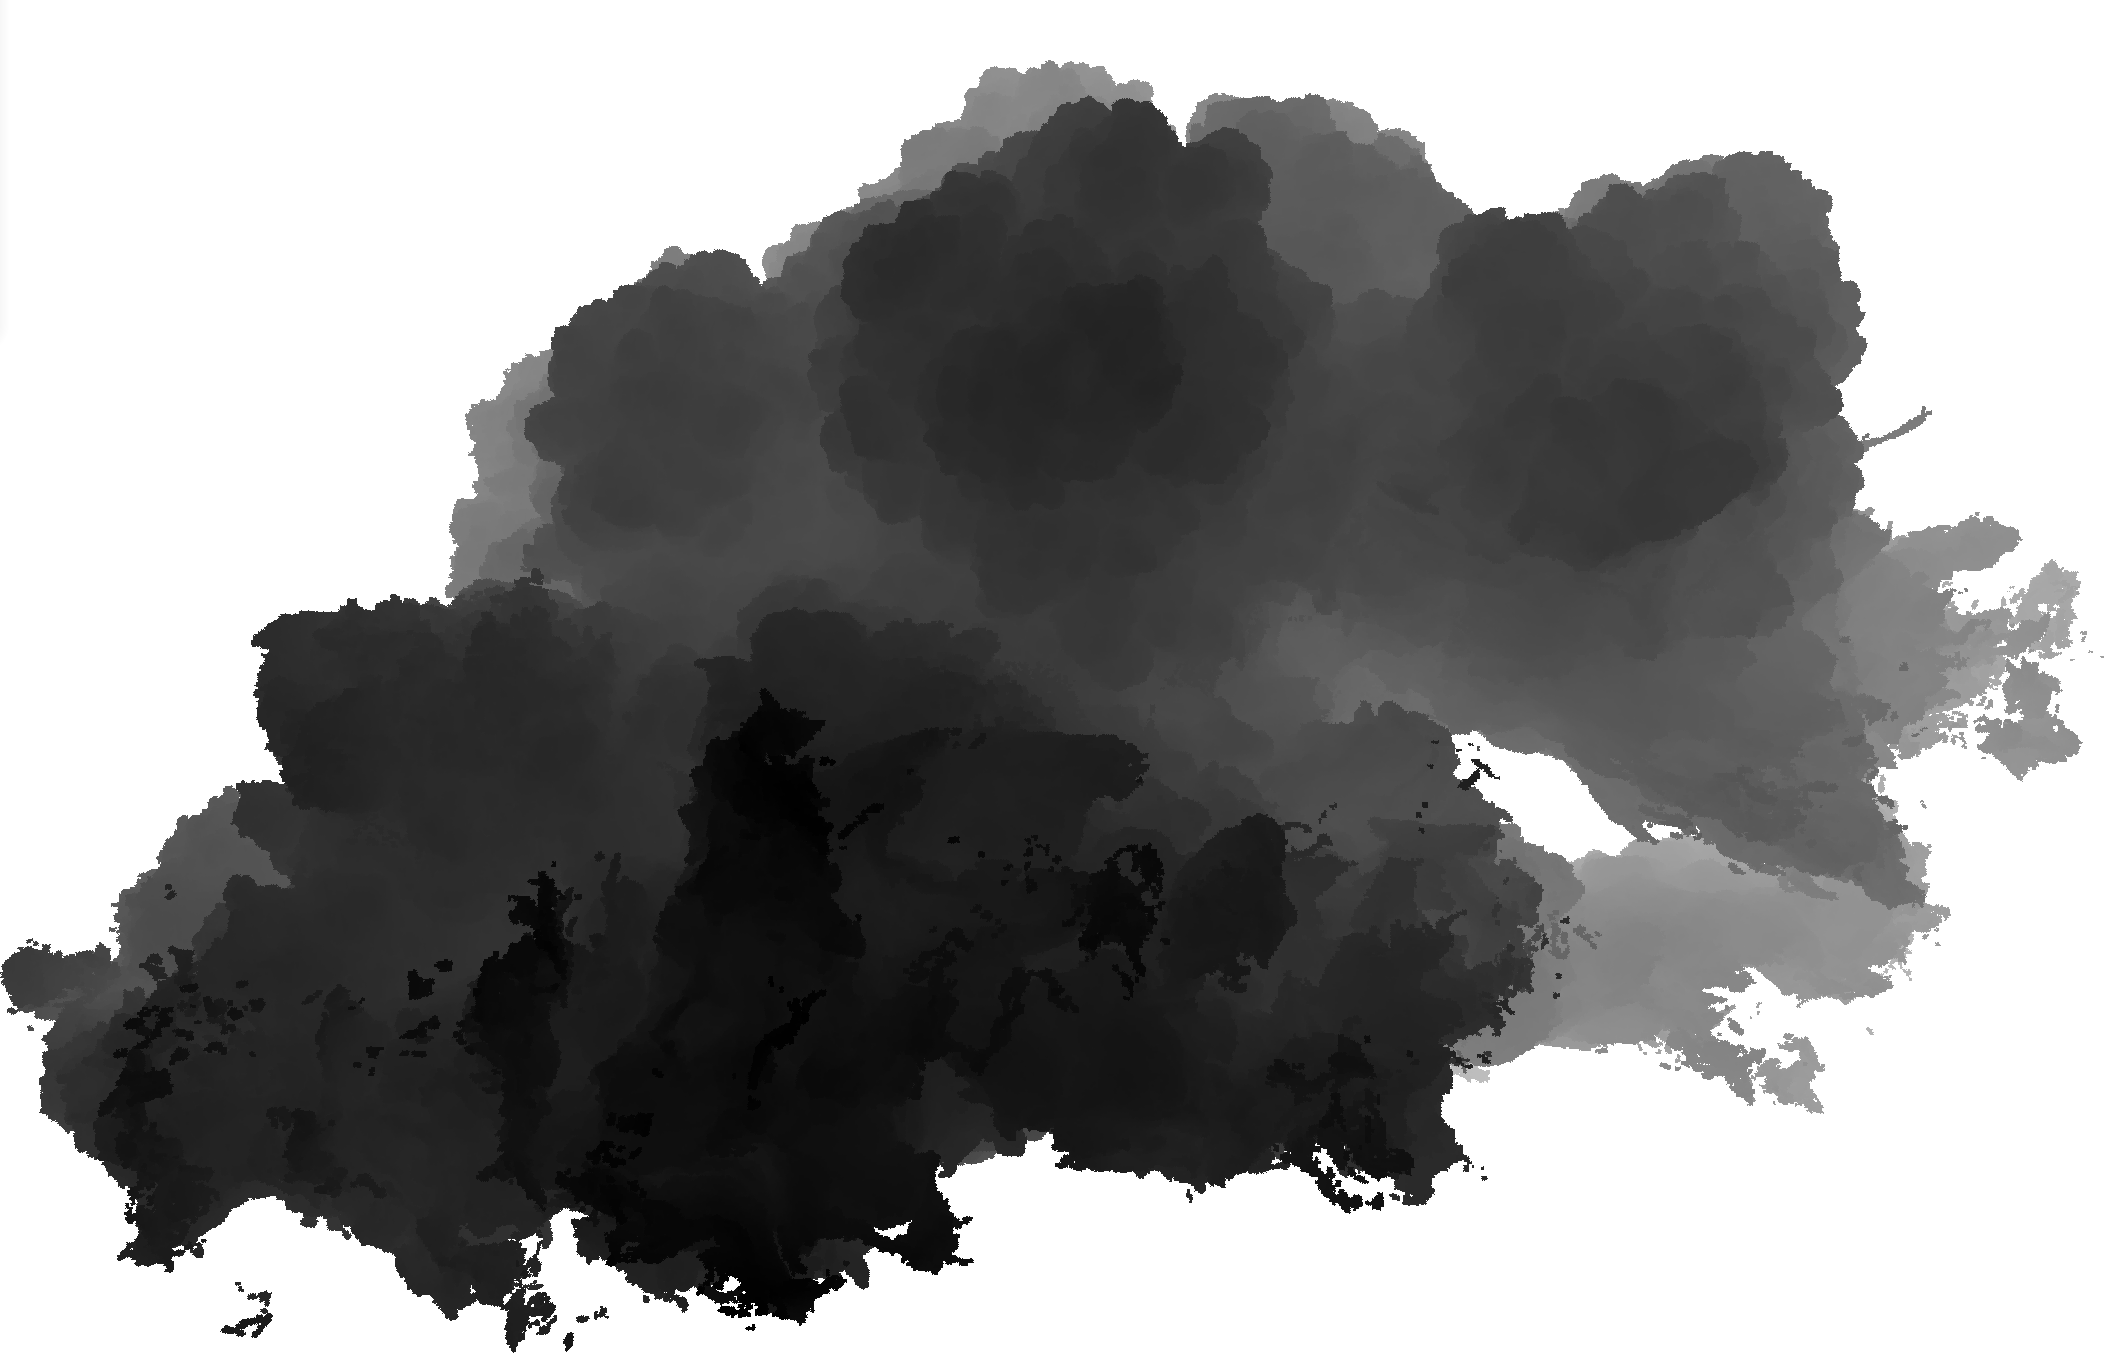
\includegraphics[width=0.45\textwidth]{figures/disney_cloud_half_res_depth.png}
    }
    \hfill
    \subfloat[Shaded by index into the voxel index. Shown is a conversion from index to hue using the following formula: $x + y\times dim\_size + z\times dim\_size^2$. The striped pattern is a result of bricks ($8^3$ voxels) are a combination of two texture slices, these are the altering index colors. The larger shifts in color, which are in specific cubic regions, correlate to the different L2 nodes.]{
        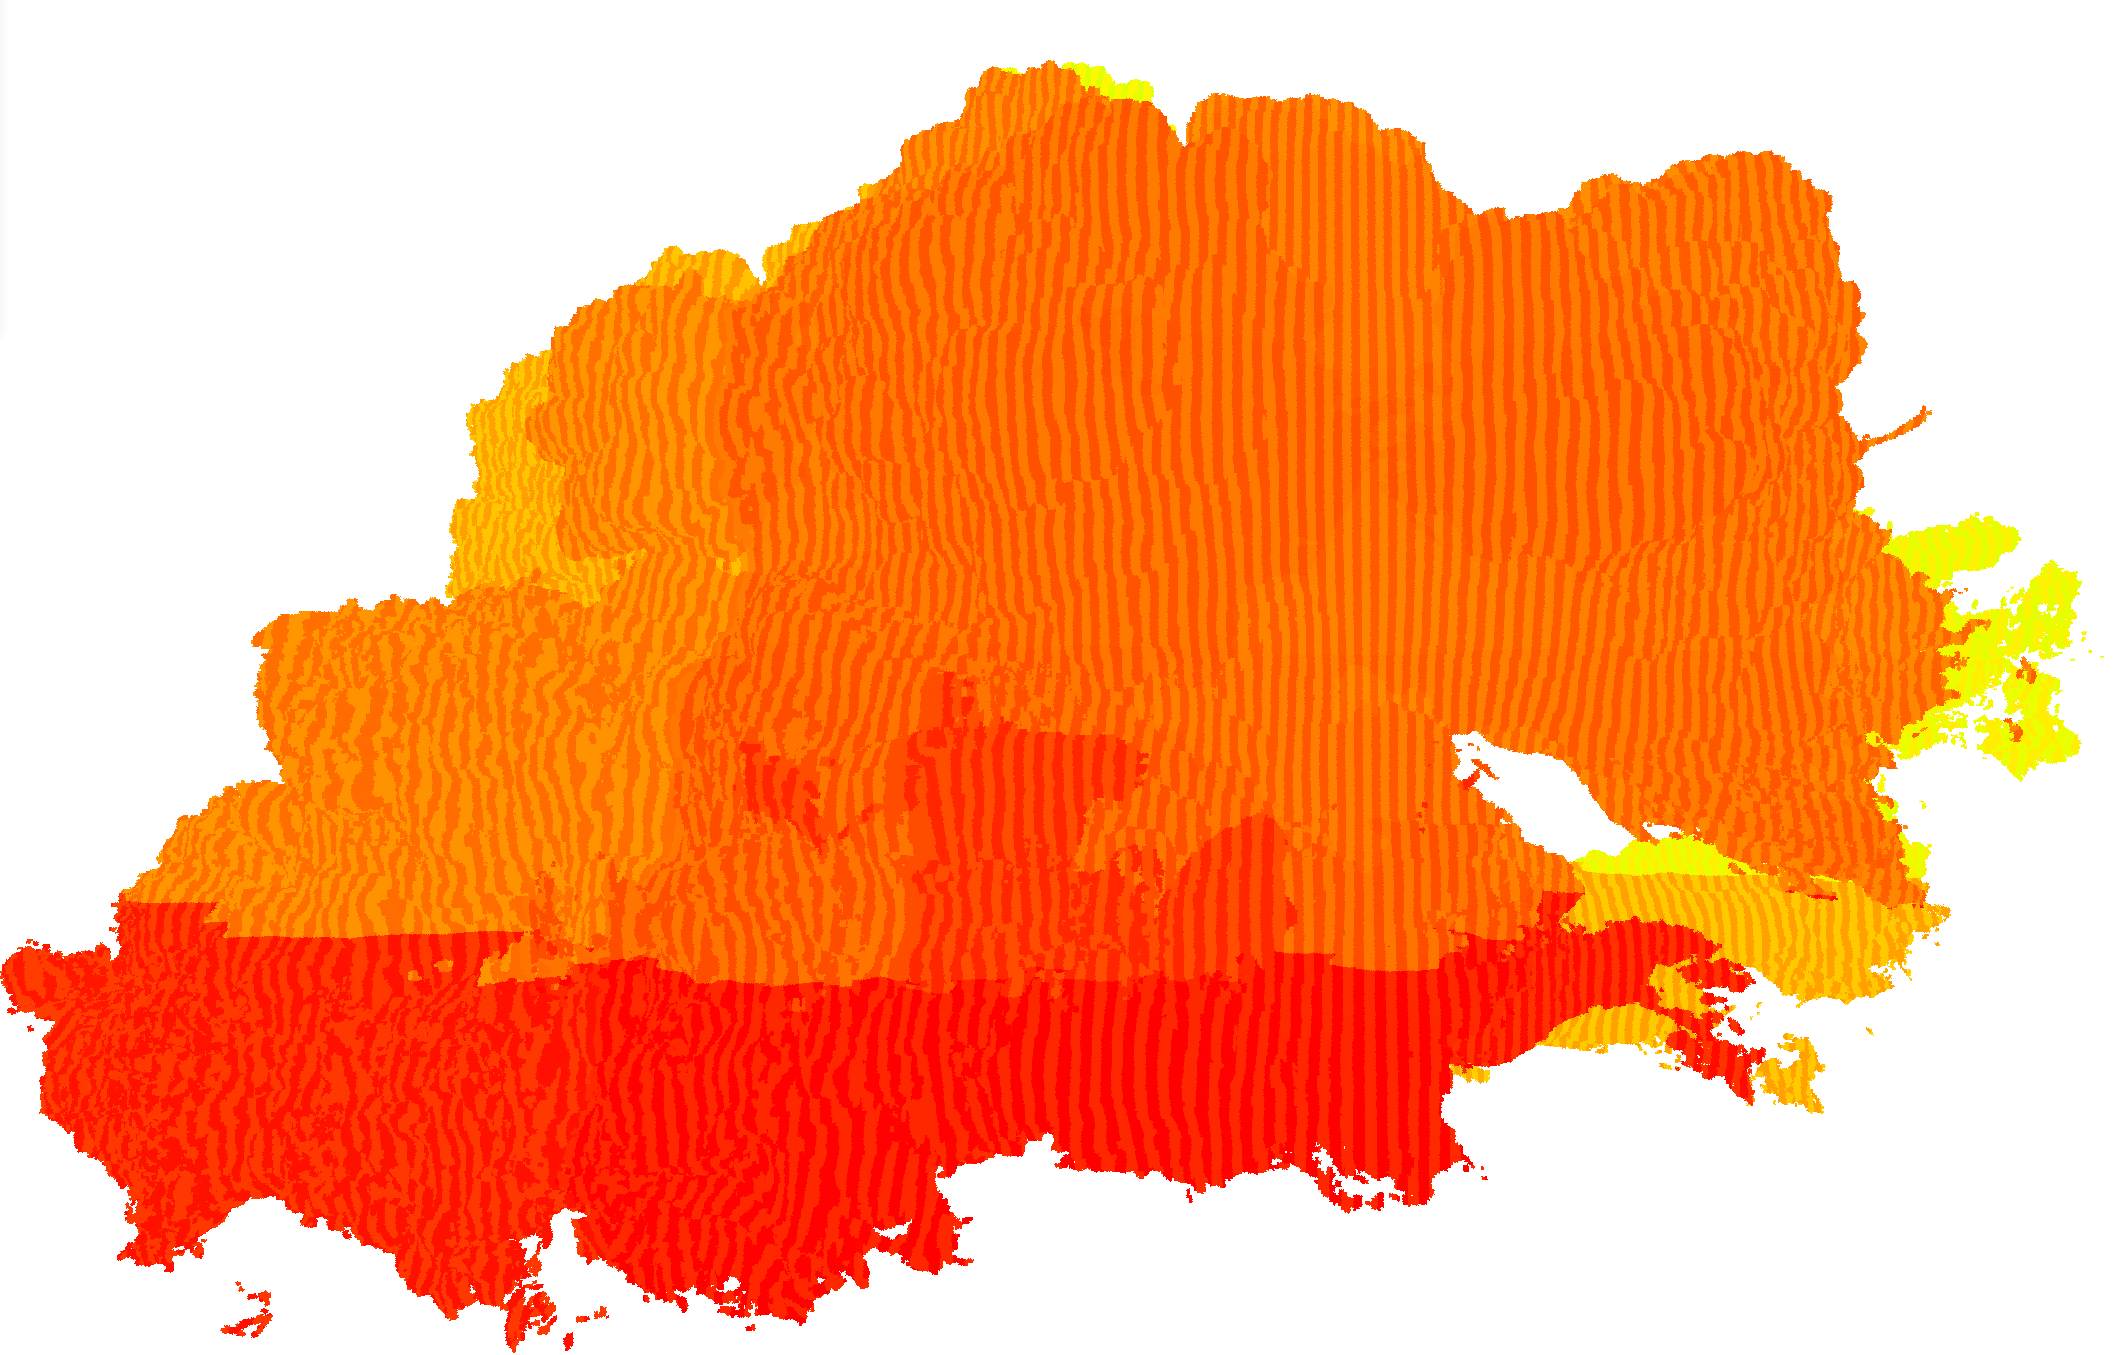
\includegraphics[width=0.45\textwidth]{figures/disney_cloud_half_res_index.png}
    }
    \hfill
    \subfloat[Shaded by the density of the first hit voxel, where a low density is red and a high density results in different hues. Overall the entire outside edge of the cloud only shows low-density voxels, but there are some spots where deeper voxels are visible which have a higher density.]{
        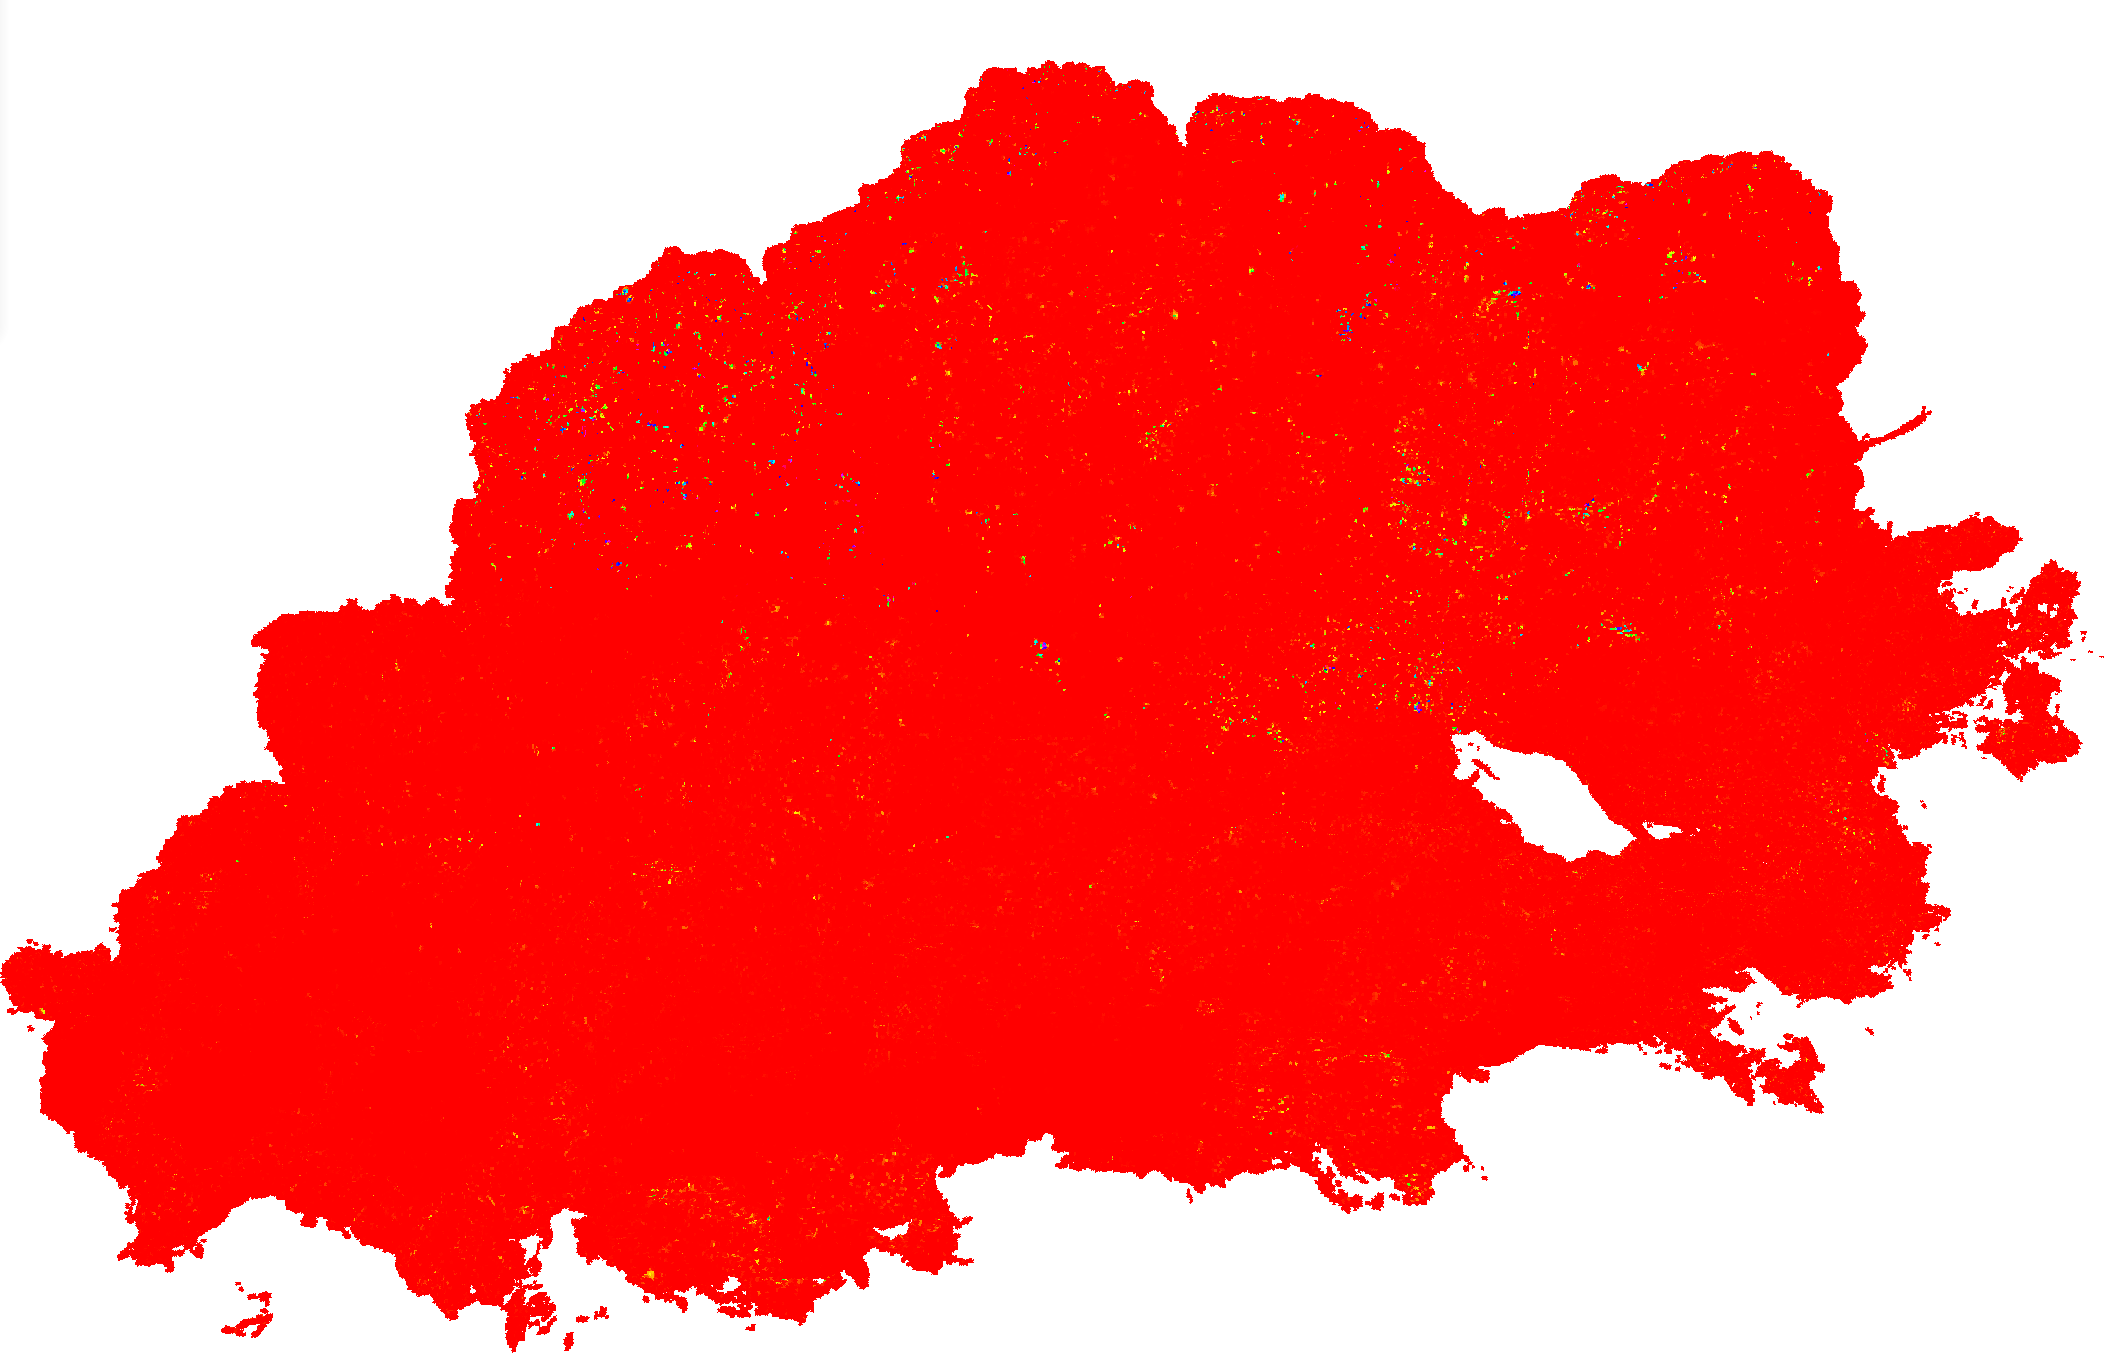
\includegraphics[width=0.45\textwidth]{figures/disney_cloud_half_res_first_temp.png}
    }
    \caption{Some shading options of the VDB viewer application. The exact color values do not matter in this example, these figures exist to illustrate general patterns. All renders are done using the half-resolution version of the Disney Cloud \cite{DisneyCloud}. } \label{implementation:vdb_viewer:debug_views}
\end{figure}
\clearpage
\section{Results} \label{results}
\clearpage
\section{Conclusion} \label{conclusion}
\clearpage


\bibliographystyle{apalike}
\bibliography{refs}

\end{document}
